\documentclass[10pt,aspectratio=169,dvipsnames]{beamer}
\usetheme[]{Berlin}

\setbeamertemplate{footline}{
  \usebeamercolor[fg]{framesource}%
  \usebeamerfont{page number in head}%
  \hspace{0.2cm}
  \small \insertframenumber
  \vspace{0.2cm}
  \doclicenseIcon
  \hfill
  
\includegraphics[height=0.8cm]{logos/tub_logo.pdf}
  \hspace{0.2cm}
}

\setbeamercovered{transparent}

\setbeamertemplate{footline}[
 myframe number]

% PACKAGES
\usepackage[absolute,overlay]{textpos}
\usepackage[utf8]{inputenc}
\usepackage[official]{eurosym}
\usepackage{booktabs}
\usepackage{parskip}
\usepackage{bm}
\usepackage{tikz}
\usepackage{adjustbox}
\usepackage[super]{nth}

\usepackage[
    type={CC},
    modifier={by},
    version={4.0},
]{doclicense}

% HYPERREFERENCES
\usepackage{hyperref}
\hypersetup{
	colorlinks=true,
	citecolor=tub-blue,
	linkcolor=tub-blue,
	urlcolor=tub-blue
}

\usepackage[sfdefault]{roboto}
\usepackage[normalem]{ulem}
\usepackage{multicol}

% GRAPHICS	
\graphicspath{
    {graphics/},
    {../workflow/notebooks/figures} % study results
    {../results/2030-targets-smr-0.5}
  }
\DeclareGraphicsExtensions{.pdf,.jpeg,.png,.jpg}

% FORMATTING
\setlength{\parskip}{6pt}
\linespread{1.1}
\newcommand{\seprule}{\par\noindent\textcolor{black!25}{\rule{\textwidth}{0.4pt}}}

% SOURCES
\setbeamercolor{framesource}{fg=gray}
\setbeamerfont{framesource}{size=\tiny}
\newcommand{\source}[1]{\begin{textblock*}{10cm}(3.6cm,8.25cm)
    \begin{beamercolorbox}[ht=0.5cm,right]{framesource}
        \usebeamerfont{framesource}\usebeamercolor[fg]{framesource} Source: {#1}
    \end{beamercolorbox}
\end{textblock*}}

% REFERENCES
% \usepackage[style=nature, doi=true, maxcitenames=3]{biblatex}
% \bibliography{bibliography}
% \renewcommand*{\bibfont}{\footnotesize}

% COLOR TEXT
\newcommand{\bl}[1]{\textcolor{tub-blue}{#1}}
\newcommand{\gr}[1]{\textcolor{tub-green}{#1}}
\newcommand{\rd}[1]{\textcolor{tub-red}{#1}}
\newcommand{\yl}[1]{\textcolor{tub-yellow}{#1}}
% \newcommand{\org}[1]{\textcolor{tub-orange}{#1}}
\newcommand{\cb}[1]{\colorbox{gray!20}{#1}}

\usepackage{array}% https://ctan.org/pkg/array
\makeatletter
\g@addto@macro{\endtabular}{\rowfont{}}% Clear row font
\makeatother
\newcommand{\rowfonttype}{}% Current row font
\newcommand{\rowfont}[1]{% Set current row font
   \gdef\rowfonttype{#1}#1%
}
\newcolumntype{L}{>{\rowfonttype}l}
\newcolumntype{R}{>{\rowfonttype}r}

% Custom commands
\usepackage{caption}
\renewcommand{\figurename}{} % Removes the "Figure" text
\captionsetup[figure]{labelformat=empty, labelsep=none} % Removes numbering and colon


% FONT
%\usepackage{utopia}

% REFERENCES
%\usepackage[backend=biber,style=authoryear-comp]{biblatex}
%\bibliography{references.bib}

% TITLE PAGE
\title{
  \textbf{ISESA}\\\nth{1} International Symposium on Energy System Analysis 
}
\vspace*{-.5cm}

% \author{STRIse}
\institute[Technische Universität Berlin] % (optional, but mostly needed)
{ 
  \normalsize
  \alert{Resilient strategies for the European energy system} \\
  \alert{A case study on 2030 EU policy targets} \\
  \footnotesize
  \textbf{Bobby Xiong}\\
  \href{mailto:xiong@tu-berlin.de}{xiong@tu-berlin.de} \\
  % Department of Digital Transformation in Energy Systems \\
  Technische Universität Berlin, Germany \\

  \vspace{0.2cm}

  November 11, 2024
}

\date{}

\subject{Recent Research with PyPSA-Eur}

\titlegraphic{%
\vspace{-1cm}

\includegraphics[height=1cm,clip=true]{logos/cetp_logo.png}
\hspace{0.5cm}
\includegraphics[height=1cm,clip=true]{logos/ensys_short_logo.pdf}
\hspace{0.5cm}
\includegraphics[trim=0 0cm 0 0cm,height=1cm,clip=true]{logos/tub_logo.pdf}
\hspace{0.5cm}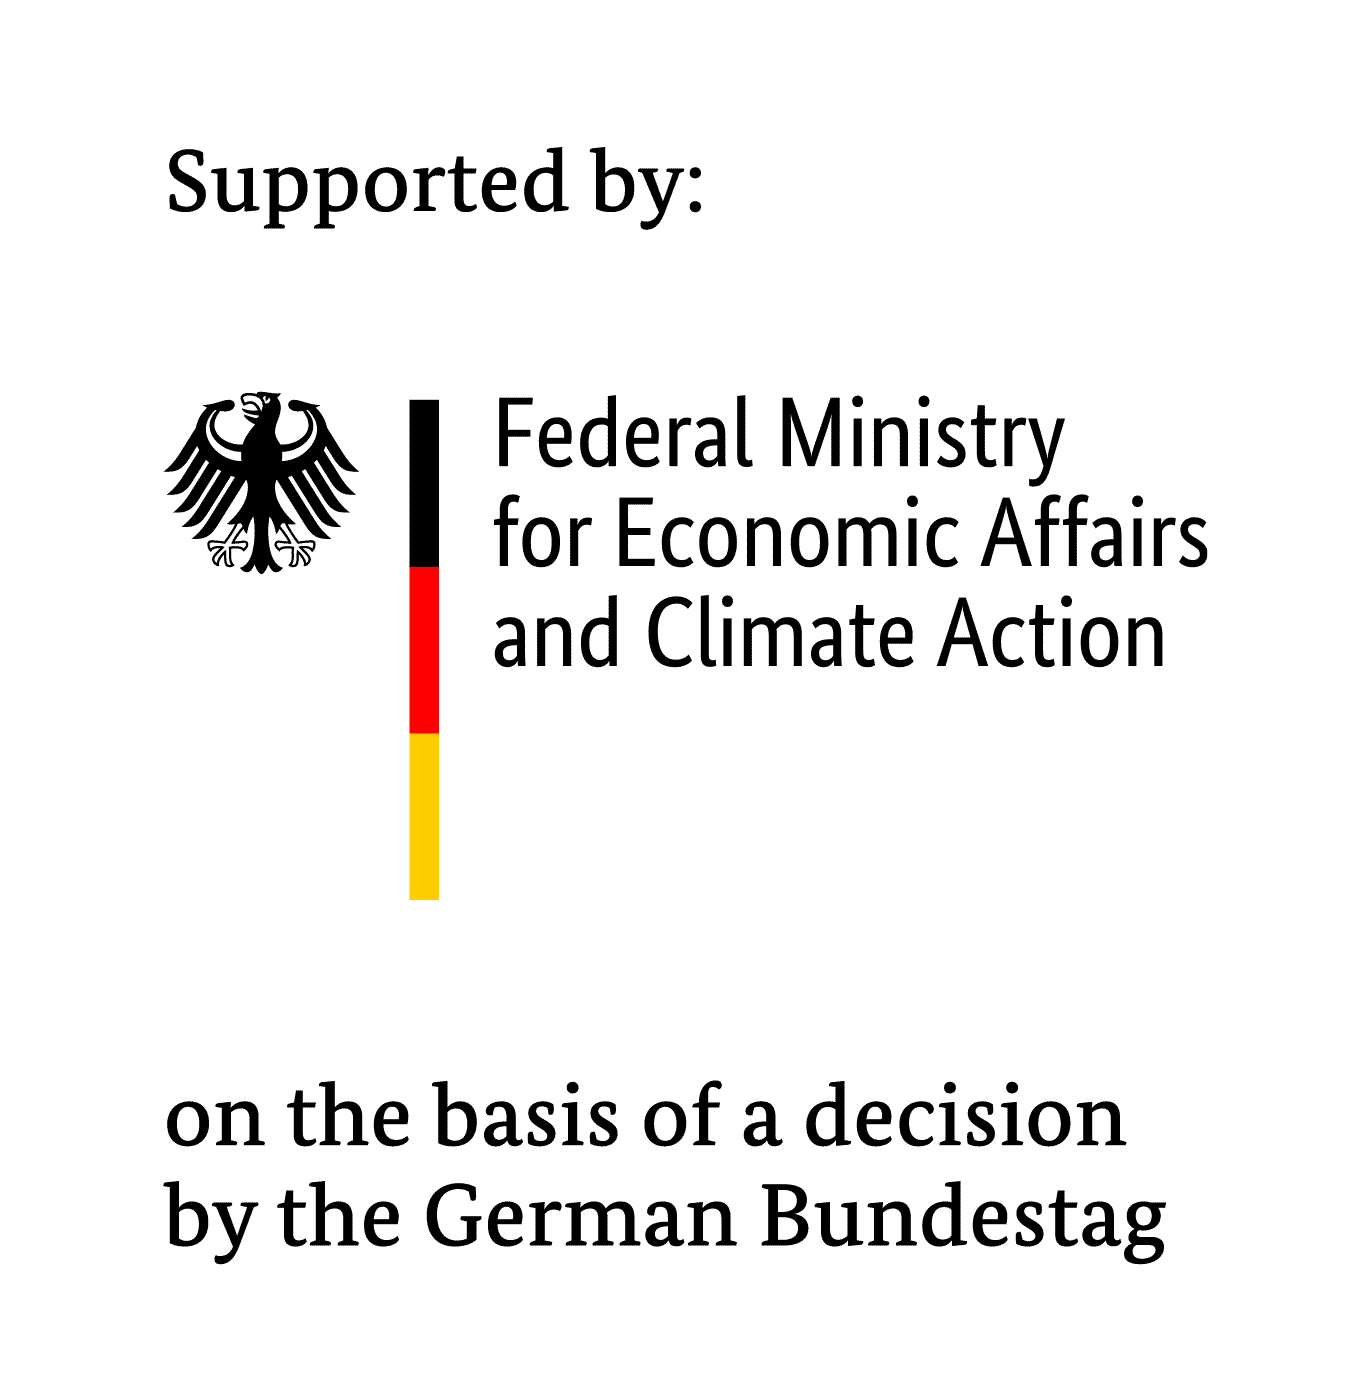
\includegraphics[trim=0.2cm 0.6cm 0.6cm 0.2cm,height=1.1cm,clip=true]{logos/bmwk_en_logo.png}
}


\begin{document}

\addtocounter{framenumber}{-1}
{
  \setbeamertemplate{footline}{
    \usebeamercolor[fg]{framesource}%
    \usebeamerfont{page number in head}%
    \begin{center}
      \Large
      \doclicenseIcon
      \vspace{0.4cm}
    \end{center}
  } 
  \maketitle
}

\section{Introduction}


\begin{frame}{RESILIENT project partners}
  \centering
  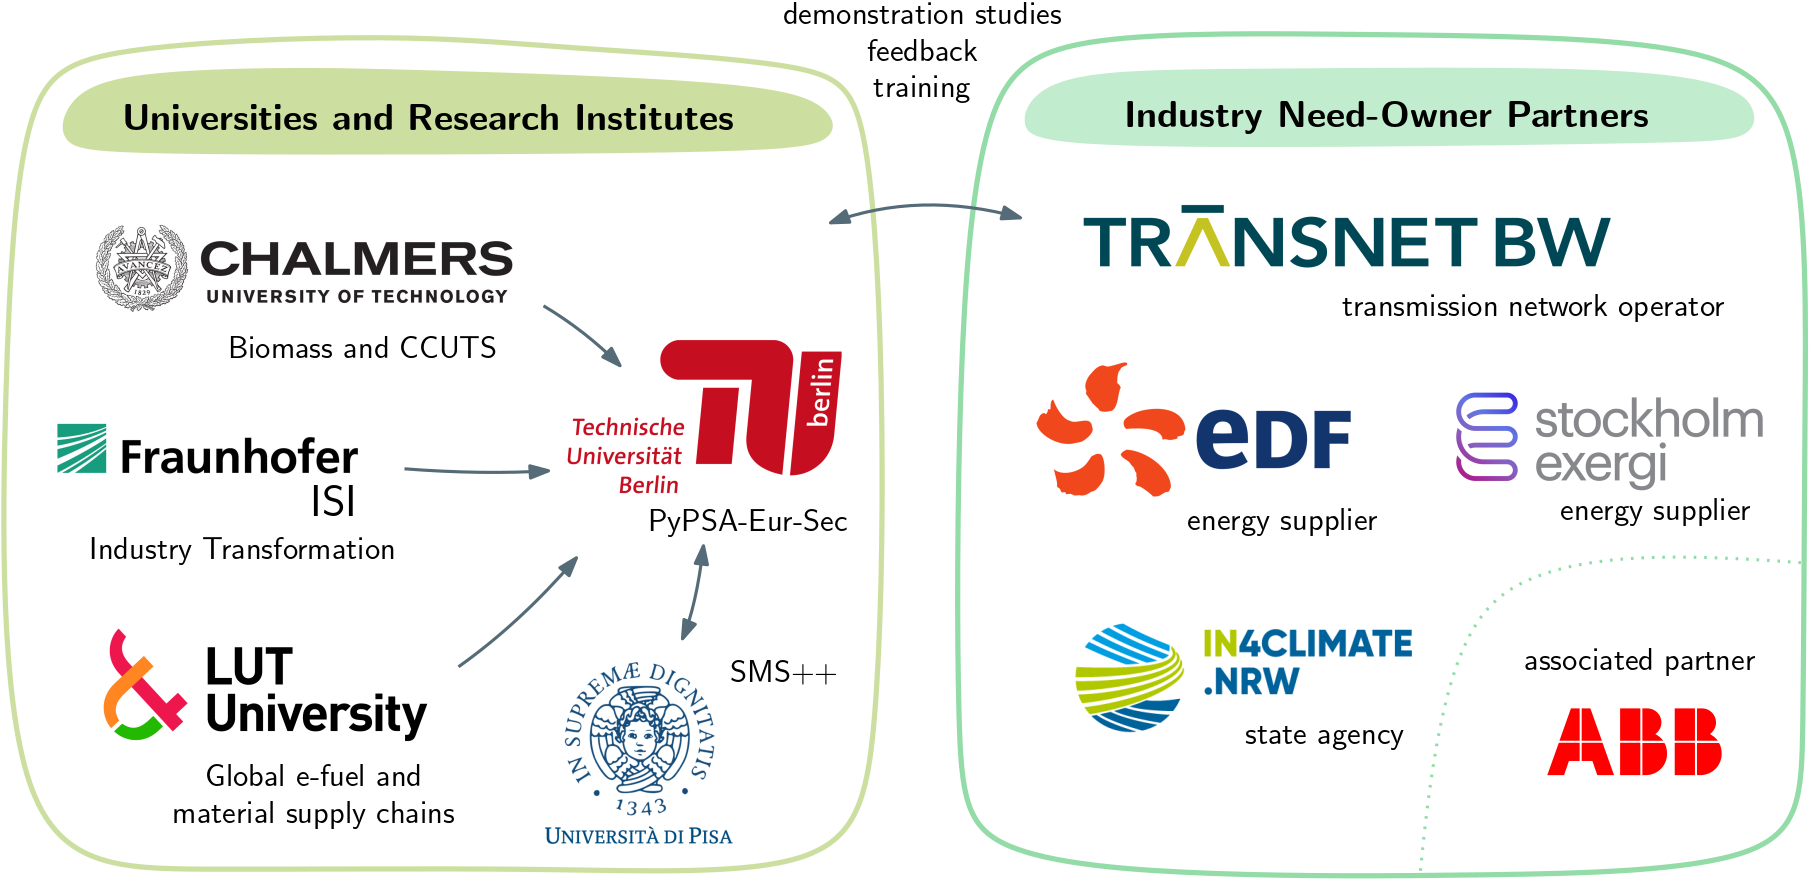
\includegraphics[width=0.85\textwidth]{other/resilient_partners}
  
  \footnotesize
  Funded via \alert{CETPartnership 2022} Call --- \alert{BMWK} for all German partners.

  \source{\url{https://resilient-project.github.io/}}
\end{frame}

\begin{frame}{RESILIENT work packages}
  \centering
  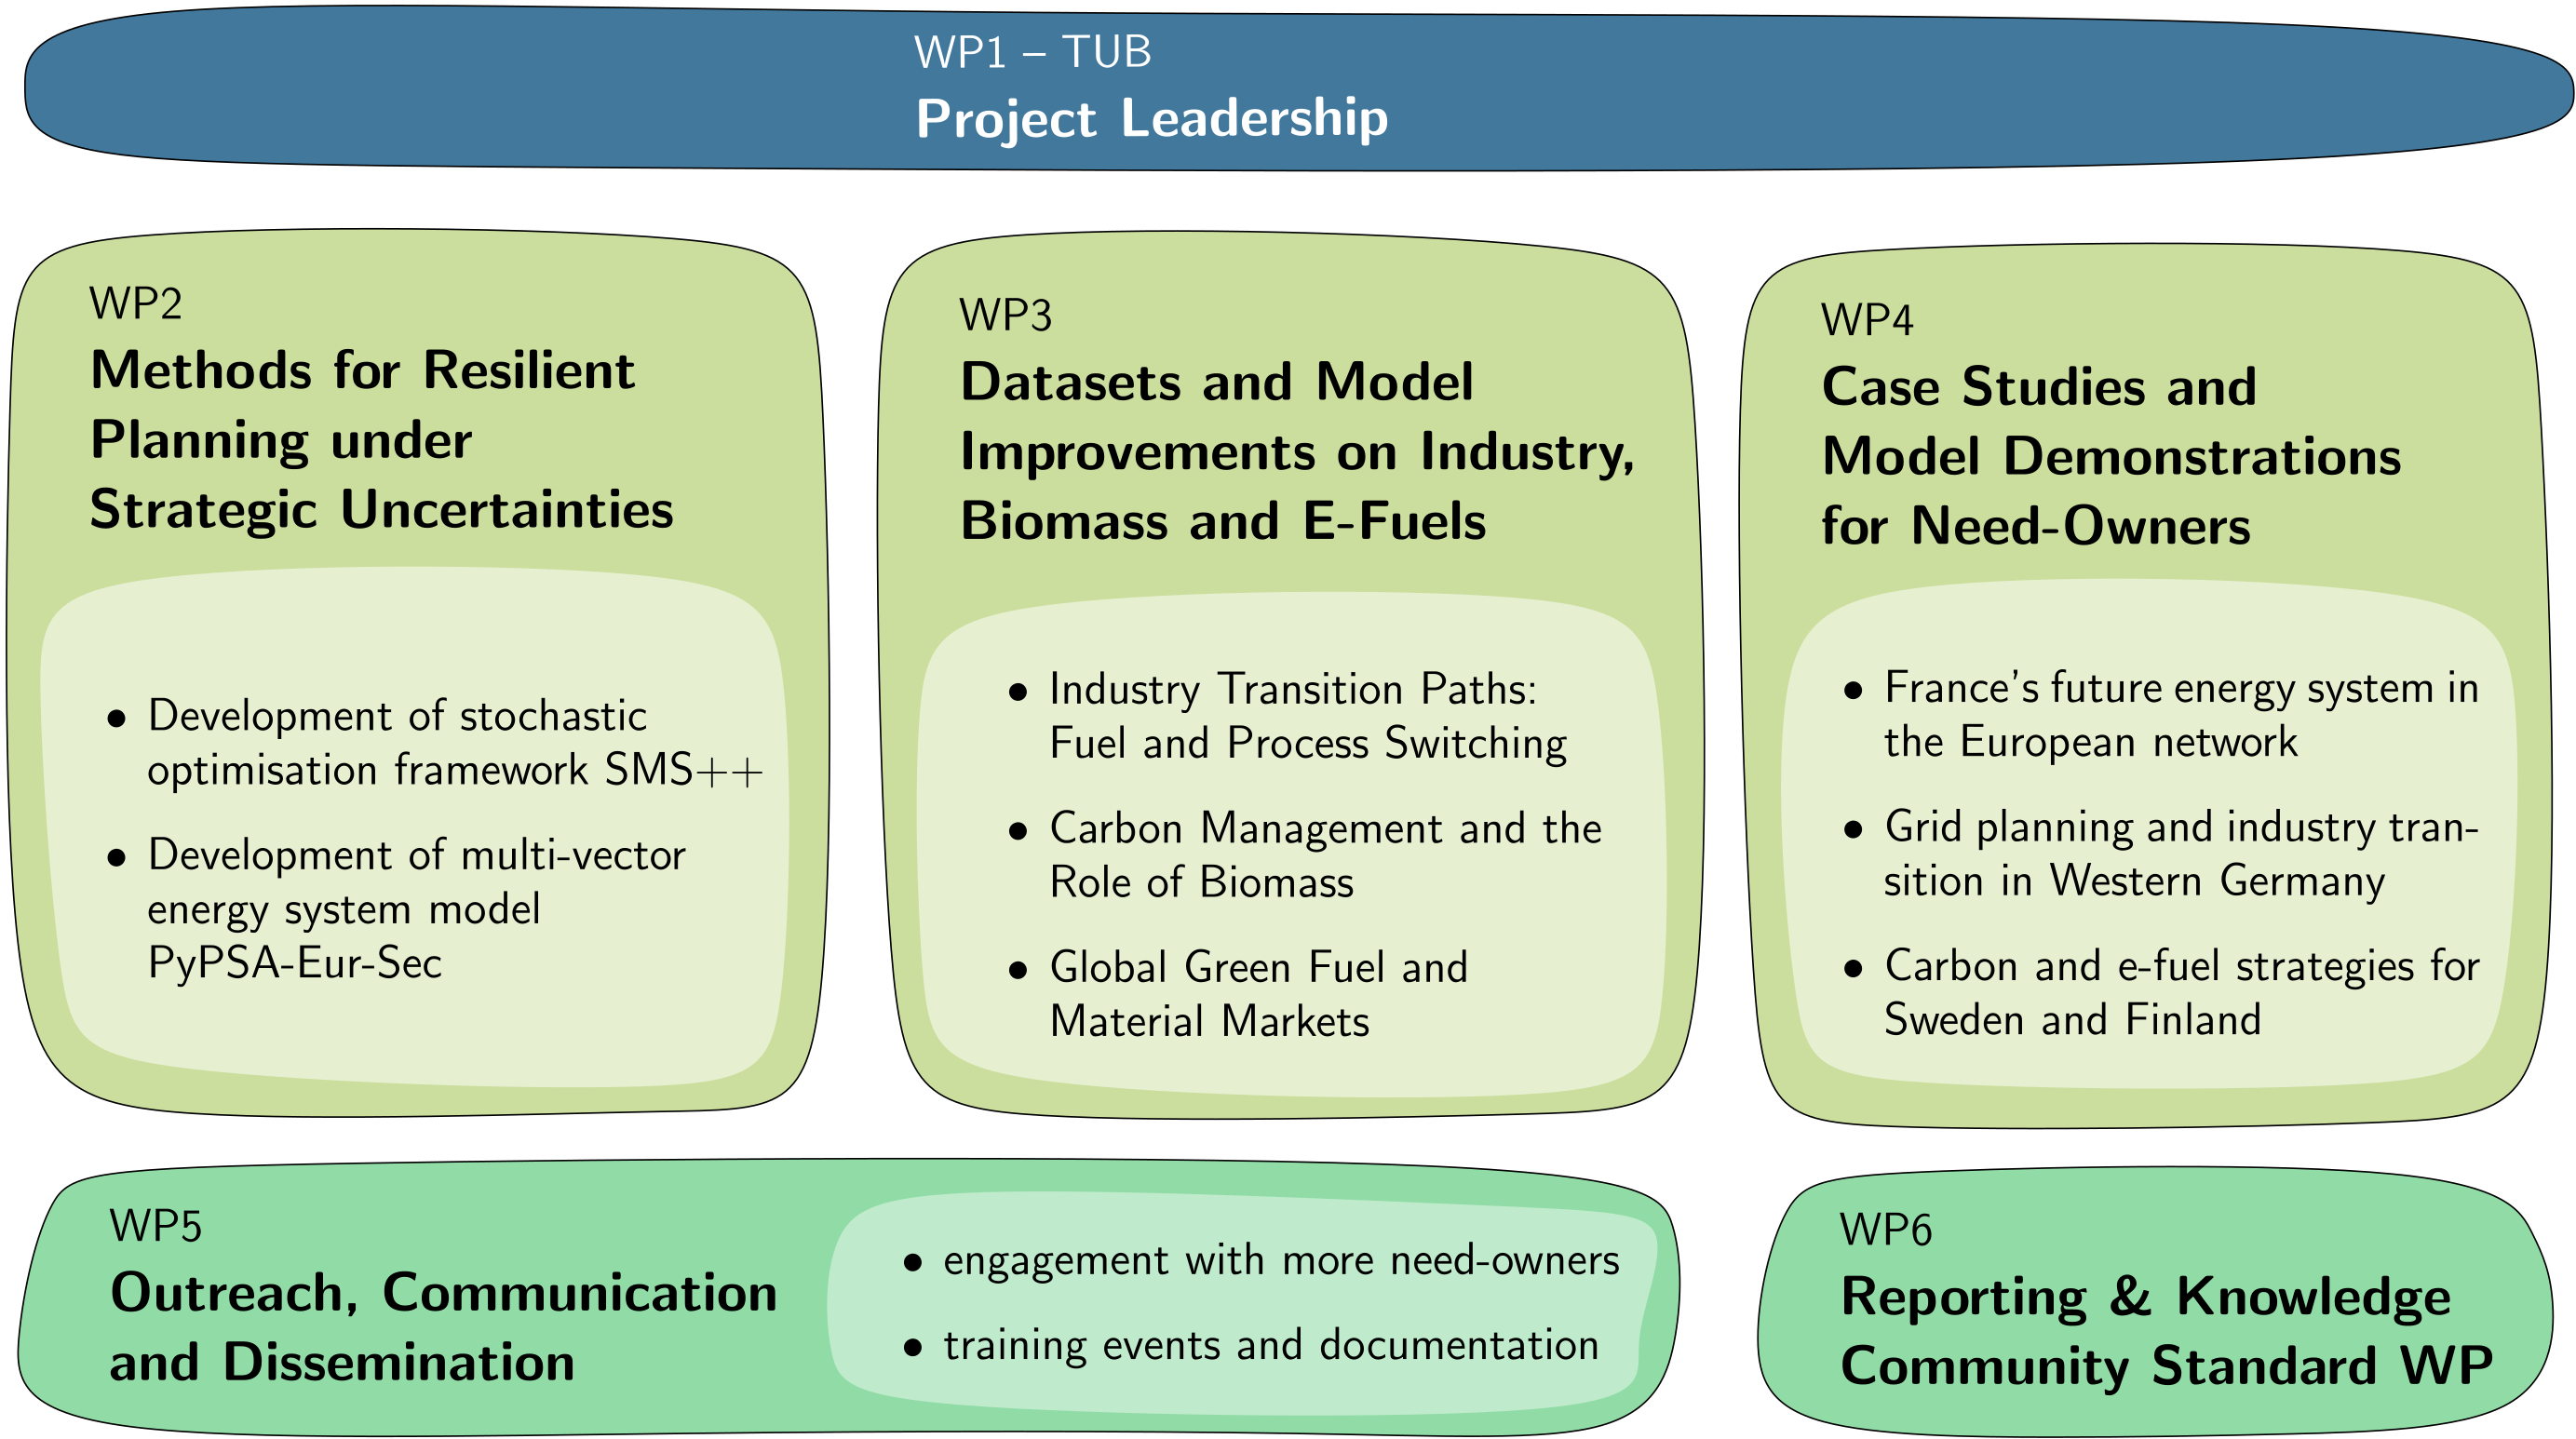
\includegraphics[width=0.8\textwidth]{other/resilient_project_structure}
\end{frame}

\begin{frame}{PyPSA-Eur: An open-source, sector-coupled model for Europe}
  \begin{columns}
    \begin{column}{0.5\textwidth}
      \footnotesize
      \begin{itemize}
        \setlength\itemsep{.8em}
        \item Spatially and temporally highly resolved linear optimisation model that covers the \alert{European} continent,
        \item Built on top of the open-source toolbox \alert{PyPSA},
        \item Includes \alert{stock} of existing power plants, renewable potentials, availability \alert{time series},
        \item Covers the \alert{electricity high-voltage grid} from AC 220 kV to 750 kV (UA) and DC 150 kV upwards, option to include planned transmission projects (TYNDP and German NEP),
        \item Maintained by the Department of Digital Transformation in Energy Systems at \alert{TU Berlin}.
      \end{itemize}
    \end{column}
    \begin{column}{0.5\textwidth}
      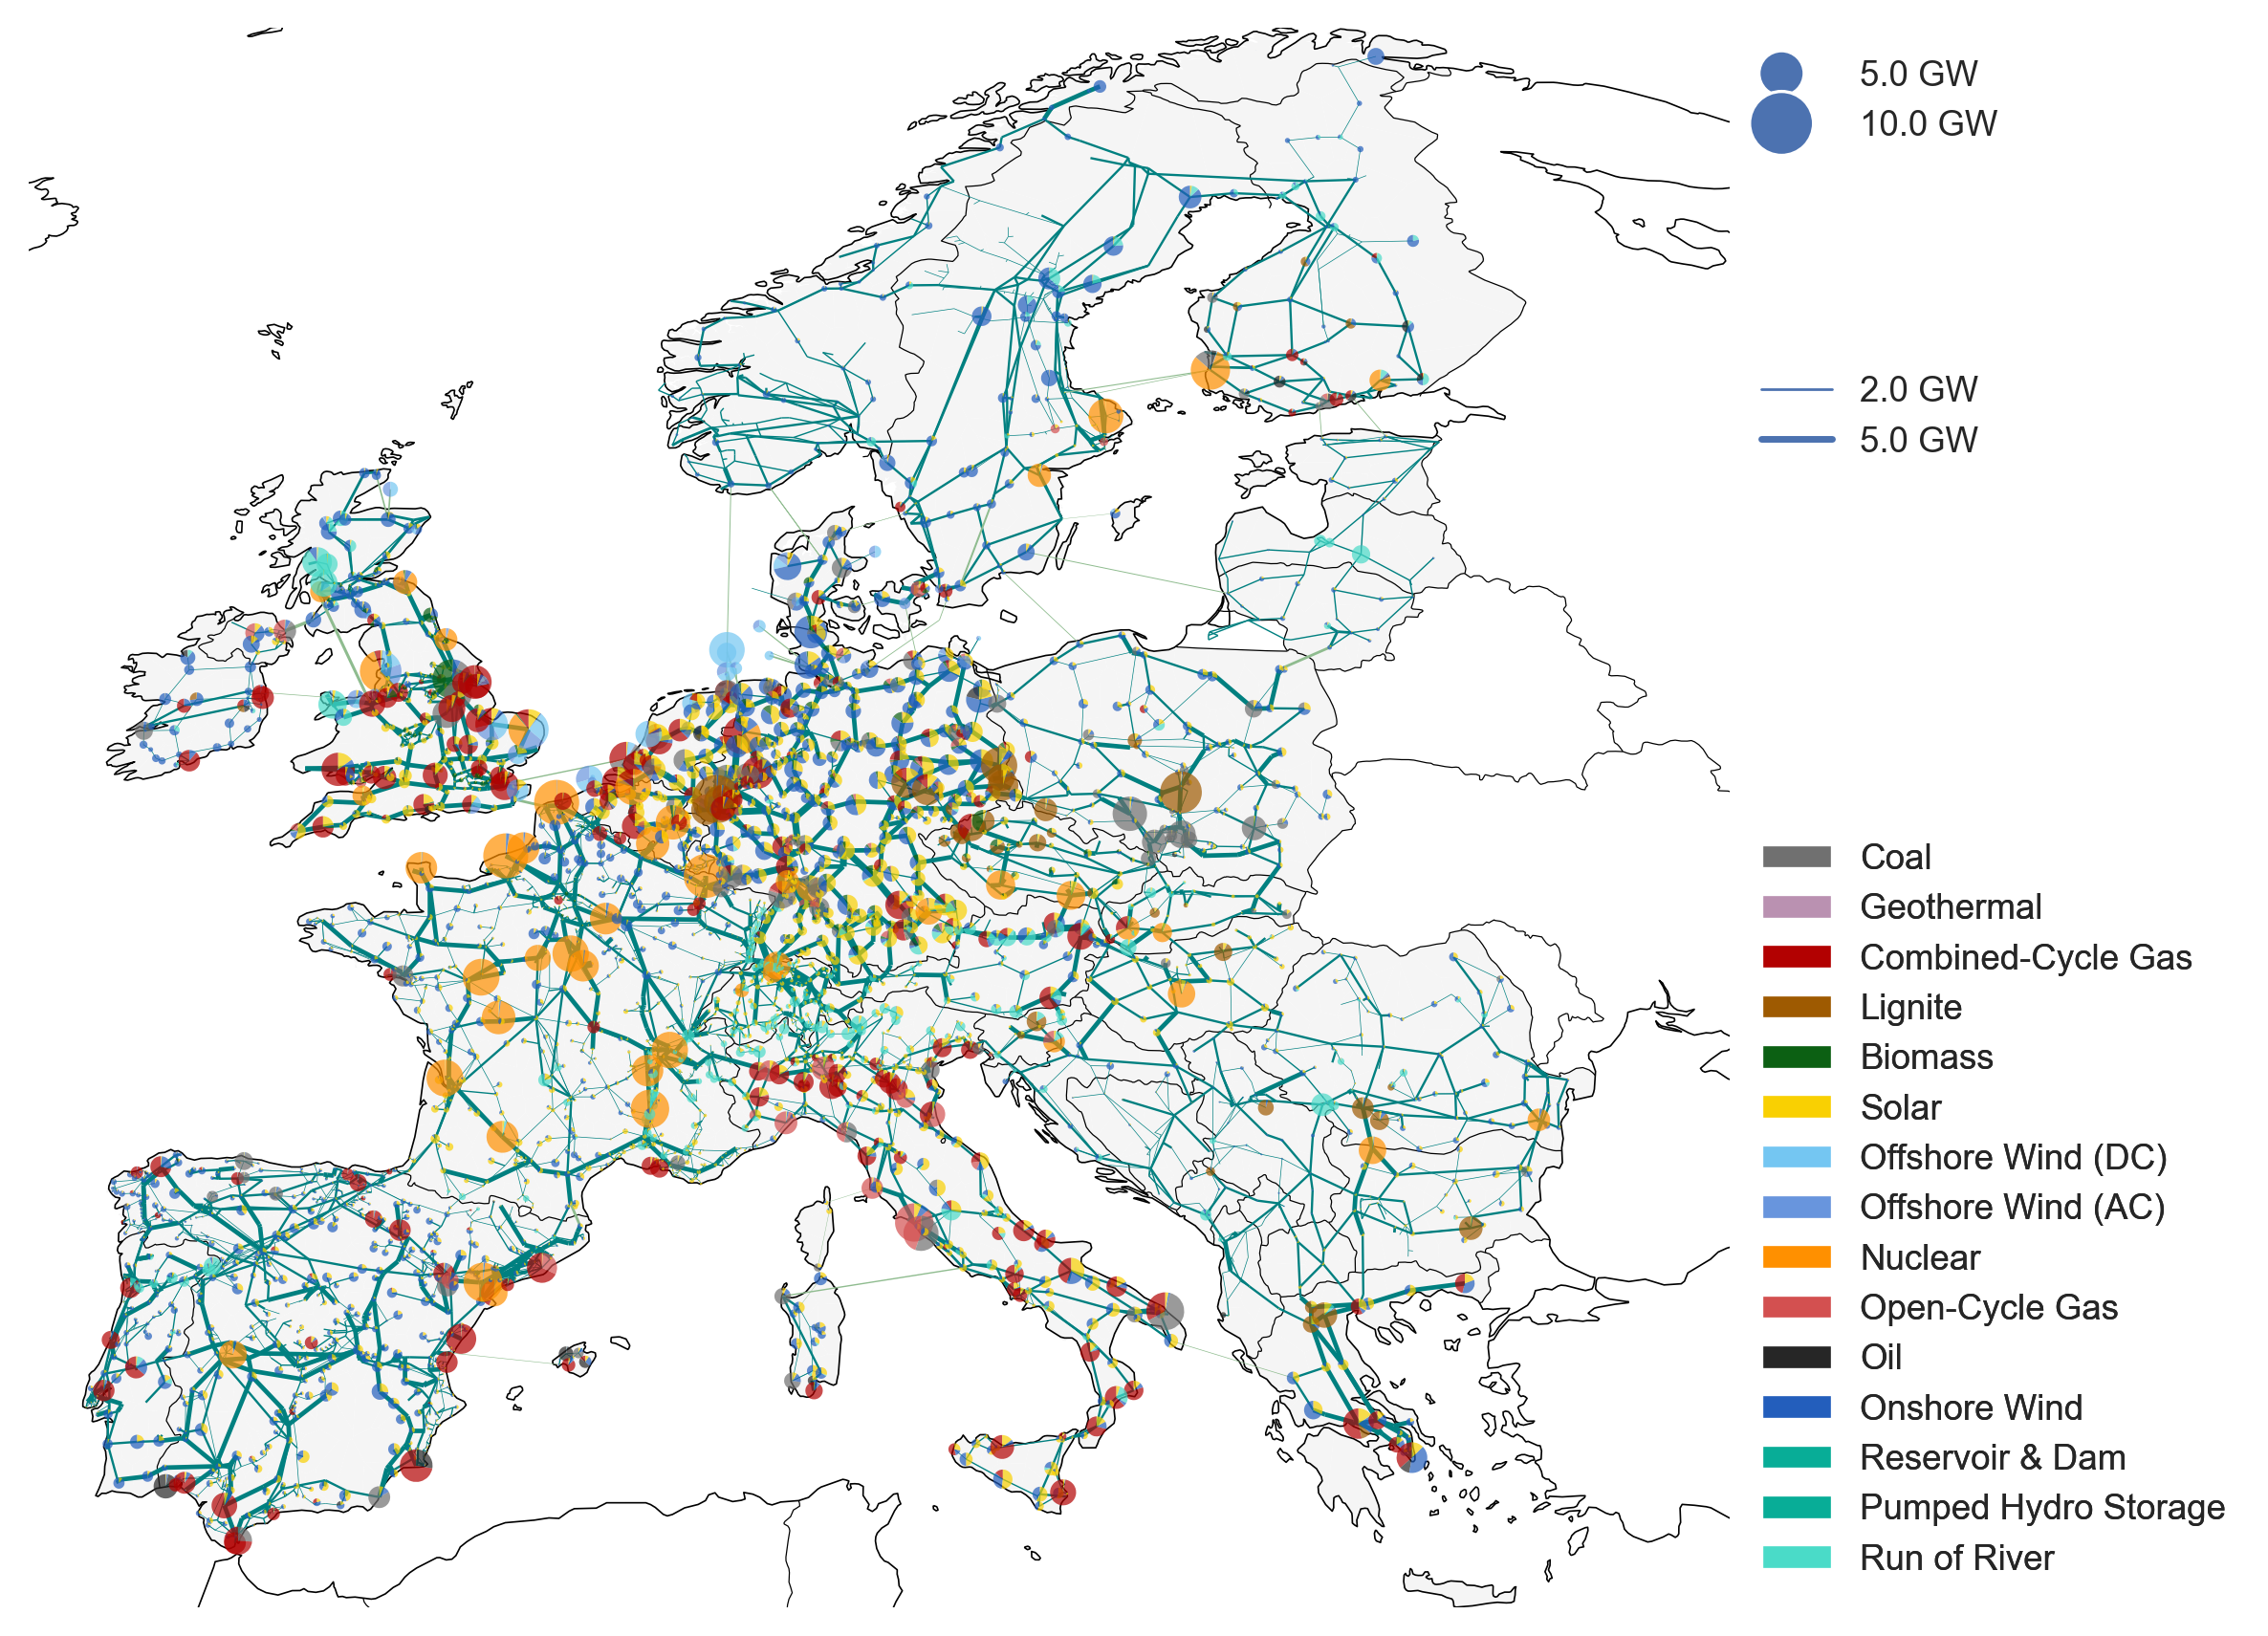
\includegraphics[width=1\textwidth]{other/pypsa_eur_elec}
    \end{column}
  \end{columns}

  \source{\url{https://pypsa-eur.readthedocs.io}}
\end{frame}

\begin{frame}{Selection of planned model developments}
  \footnotesize
  \begin{columns}[T] % align columns
    \begin{column}{.5\textwidth}
        \begin{minipage}[t][.45\textheight]{\linewidth}
            \begin{alertblock}{\textbf{Computational methods for uncertainties}}
                \begin{itemize}
                  \item decomposition techniques
                  \item large-scale stochastic optimisation
                  \item \textbf{test robustness of system}
                  \item using SMS++ framework
                \end{itemize}
            \end{alertblock}
        \end{minipage}
        
        \vspace{-0.03\textheight} % separation between the boxes
        
        \begin{minipage}[t][.45\textheight]{\linewidth}
            \begin{alertblock}{\textbf{Industry transformation (FORECAST)}}
              \begin{itemize}
                \item fuel and process switching
                \item industry relocation
                \item carbon sources and feedstocks
                \item data on stock \& investment cycles
                \item new technologies (oxyfuel cement, etc.)
              \end{itemize}
            \end{alertblock}
        \end{minipage}
    \end{column}
    
    \begin{column}{.5\textwidth}
        \begin{minipage}[t][.45\textheight]{\linewidth}
            \begin{alertblock}{\textbf{Carbon management and biomass usage}}
              \begin{itemize}
                \item \textbf{CO$_2$ network}
                \item \textbf{CO$_2$ sequestration potentials}
                \item circular carbon economy and recycling
                \item biomass usage options
              \end{itemize}
            \end{alertblock}
        \end{minipage}
        
        \vspace{-0.03\textheight} % separation between the boxes
        
        \begin{minipage}[t][.45\textheight]{\linewidth}
            \begin{alertblock}{\textbf{Global green fuel and material markets}}
              \begin{itemize}
                \item \textbf{imports of green energy and materials}
                \item \textbf{effects on European infrastructure}
                \item restructuring of value chains
                \item risks (geopolitical, technological, etc.) \newline
              \end{itemize}
            \end{alertblock}
        \end{minipage}
    \end{column}
\end{columns}
\end{frame}

\section{Case study setup}
\begin{frame}{Case study: Motivation and research questions}
  \footnotesize

  The EU has set ambitious targets for 2030, including the electricity, hydrogen and CO$_2$ infrastructure sector.

  \begin{columns}[T] % align columns
    % First column
    \begin{column}{.3\textwidth}
        \begin{minipage}[t][.45\textheight]{\linewidth}
            \begin{alertblock}{\textbf{55 \% emission reduction}}
                \begin{itemize}
                  \item \alert{Fit for 55}
                  \item Translating to an emission allowance of ca. 2 bn. t CO$_2$ p.a. in 2030
                  \item Covering the electricity, heat, industry, transport, buildings and agriculture sectors \newline
                \end{itemize}
                \vspace{0.06cm}
            \end{alertblock}
        \end{minipage}
    \end{column}
    
    % Second column
    \begin{column}{.34\textwidth}
        \begin{minipage}[t][.45\textheight]{\linewidth}
            \begin{exampleblock}{\textbf{10 Mt p.a. green H$_2$ production}}
                \begin{itemize}
                  \item \alert{REPowerEU}
                  \item Accelerating the transition away from fossil fuels (esp. Russian gas), enhancing energy security through renewables
                  \item Aligns with European Green Deal and targets scaling up renewable H$_2$ in hard-to-electrify-sectors
                \end{itemize}
            \end{exampleblock}
        \end{minipage}
    \end{column}

    % Third column
    \begin{column}{.3\textwidth}
        \begin{minipage}[t][.45\textheight]{\linewidth}
            \begin{exampleblock}{\textbf{50 Mt p.a. CO$_2$ sequestration}}
                \begin{itemize}
                  \item \alert{Net-Zero Industry Act}
                  \item Essential component in helping industries to reduce their net emissions
                  \item Provides means to capture unavoidable emissions from hard-to-abate sectors like cement, steel, chemicals, etc.
                \end{itemize}
            \end{exampleblock}
        \end{minipage}
    \end{column}
  \end{columns}

  \vspace{1.3cm}

\end{frame}

\begin{frame}{Case study: Motivation and research questions}
  \scriptsize
  \begin{columns}[T] % align columns
    % First column
    \begin{column}{.63\textwidth}
        \begin{minipage}[t][.45\textheight]{\linewidth}
            \begin{alertblock}{\textbf{What are PCI-PMI projects?}}
                \begin{itemize}
                  \setlength\itemsep{0.85em}
                  \item Projects of Common Interest (PCIs) are key \alert{cross-border infrastructure projects} that link the energy systems of EU countries
                  \item Projects of Mutual Interest (PMIs) include cooperations with countries outside the EU
                  \item Intend ``to help the EU achieve its \alert{energy policy and climate objectives}: affordable, secure and sustainable energy for all citizens and the long-term decarbonisation of the economy in accordance with the \alert{Paris Agreement}''
                  \item ``Potential overall benefits of the project must outweigh its costs'' 
                  \item Given their \alert{lighthouse character}, these projects are highly likely to be implemented. 
                  \item Large infrastructure projects (incl. PCI-PMI) are however commonly facing delays due to permitting, procurement bottlenecks, etc.
                \end{itemize}
            \end{alertblock}
        \end{minipage}
    \end{column}
    
    % Second column
    \begin{column}{.36\textwidth}
        \begin{minipage}[t][.45\textheight]{\linewidth}
            \begin{alertblock}{\textbf{Project map}}
              \centering
              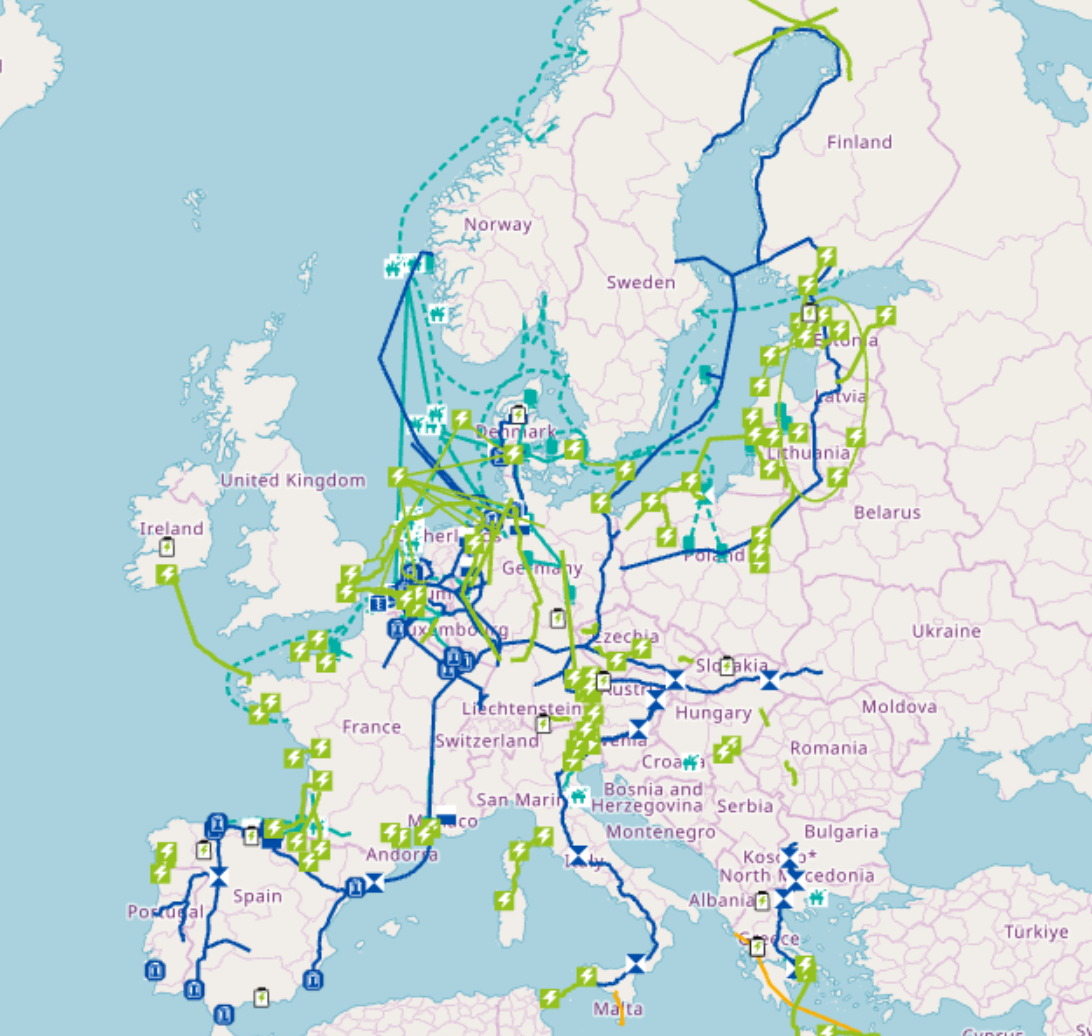
\includegraphics[width=1\textwidth]{pci_pmi_map}
            \end{alertblock}
        \end{minipage}
    \end{column}

  \end{columns}

  \vspace{2.2cm}

  \begin{enumerate}
    \item At \alert{what cost} do we stick to the targets? How does a \alert{delay of PCI-PMI projects} affect the system?
    \item What is the \alert{impact} of \alert{missing} the EU 2030 policy targets for \alert{CO$_2$ sequestration} and \alert{H$_2$ production}?
  \end{enumerate}

  \source{\url{https://energy.ec.europa.eu/topics/infrastructure_en} \\ and \url{https://ec.europa.eu/energy/infrastructure/transparency_platform/map-viewer}}

\end{frame}


\begin{frame}{Case study: Model setup}
  \begin{columns}
    \begin{column}{0.55\textwidth}
      \footnotesize
      \begin{itemize}
        \setlength\itemsep{.8em}
        \item Including sectors \alert{power, heat, transport, industry, feedstock} and \alert{agriculture}
        \item Minimising \alert{total system costs} (investment and operation) for the target year \alert{2030}
        \item \alert{Co-optimising} generation, transmission, storage, and power-to-X conversion
        \item Resolving 34 countries to \alert{90 regions} at \alert{3-hourly} temporal resolution
        \item Implementing \alert{PCI-PMI} HVAC, HVDC, hydrogen and carbon infrastructure projects as well as key \alert{policy targets}:
        \vspace{0.1cm}
        \begin{itemize}
          \scriptsize
          \item 55 \% emission reduction (\alert{Fit for 55})
          \item 10 Mt p.a. production of hydrogen (\alert{REPowerEU})
          \item 50 Mt p.a. of CO$_2$ sequestration (\alert{Net-Zero Industry Act})
        \end{itemize}
      \end{itemize}
    \end{column}
    \begin{column}{0.45\textwidth}
      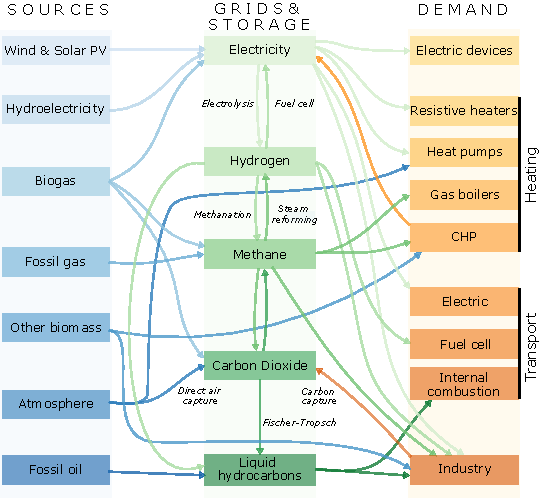
\includegraphics[width=0.95\textwidth]{other/multisector_diagram}
    \end{column}
  \end{columns}
  \source{\url{https://pypsa-eur.readthedocs.io}}
\end{frame}

\begin{frame}{Case study: Scenario setup}
  \vspace{-2.1cm}
  \footnotesize
  \begin{columns}
    \begin{column}{.31\textwidth}
      \begin{minipage}[t][.45\textheight]{\linewidth}
        \begin{alertblock}{\textbf{Base}\\(All targets)}
          \scriptsize
          \begin{itemize}
            \item \alert{Including PCI-PMI} HVAC, HVDC, H$_2$ and CO$_2$ infrastructure projects with a planned commissioning date by 2030
            \item Including exogenous CO$_2$ sequestration and H$_2$ storage sites
            \item Endogeneous expansion of CO$_2$ pipelines and national H$_2$ pipelines 
            \item Endogeneous expansion of H$_2$ storage sites
            \item 55 \% emission reduction target
            \item 10 Mt p.a. H$_2$ production target
            \item 50 Mt p.a. CO$_2$ sequestration target
          \end{itemize}
        \end{alertblock}
      \end{minipage}
    \end{column}

    % Second column
    \begin{column}{.31\textwidth}
        \begin{minipage}[t][.45\textheight]{\linewidth}
          \begin{exampleblock}{\textbf{Scenario A. PCI-PMI delay}\\(All targets)}
            \scriptsize
            \begin{itemize}
              \item \alert{Delay of all PCI-PMI projects}, no H$_2$ and CO$_2$ pipelines will be ready by 2030
              \item \alert{Endogeneous expansion of H$_2$ storage sites and CO$_2$ sequestration sites} -- according to technical sequestration potential (Hofmann et al., 2024)
              \item 55 \% emission reduction target
              \item 10 Mt p.a. H$_2$ production target
              \item 50 Mt p.a. CO$_2$ sequestration target
            \end{itemize}
          \end{exampleblock}
        \end{minipage}
    \end{column}

    % Third column
    \begin{column}{.31\textwidth}
        \begin{minipage}[t][.45\textheight]{\linewidth}
          \begin{exampleblock}{\textbf{Scenario B. PCI-PMI delay}\\(Emission target only)}
            \scriptsize
            \begin{itemize}
              \item \alert{Delay of all PCI-PMI projects, no H$_2$ and CO$_2$ pipelines will be ready by 2030}
              \item \alert{Dropping H$_2$ production and CO$_2$ sequestration targets}
              \item \alert{Endogeneous expansion of H$_2$ storage sites and CO$_2$ sequestration sites} -- according to technical sequestration potential (Hofmann et al., 2024)
              \item 55 \% emission reduction target
            \end{itemize}
          \end{exampleblock}
        \end{minipage}
    \end{column}
  \end{columns}

\end{frame}

\begin{frame}{Case study: Base --- Modelled PCI-PMI H$_2$ and CO$_2$ infrastructure}

  \begin{columns}
    \begin{column}{0.53\textwidth}
      \footnotesize
      \begin{itemize}
        \setlength\itemsep{.8em}
        \item \textbf{Base} scenario incorporates \alert{PCI-PMI} projects for \alert{H$_2$} and \alert{CO$_2$} infrastructure, including pipelines, storages (H$_2$) and sequestration sites (CO$_2$), as well as new/upgraded \alert{high-voltage AC} and \alert{high-voltage DC} lines \alert{commissioned by 2030}
        \item Total CO$_2$ sequestration capacity sums up to \alert{75 Mt p.a.}, mostly located in the North Sea
        \item Total H$_2$ storage capacity sums up to \alert{977 GWh$_{H_2}$}
      \end{itemize}
    \end{column}
    \begin{column}{0.47\textwidth}
      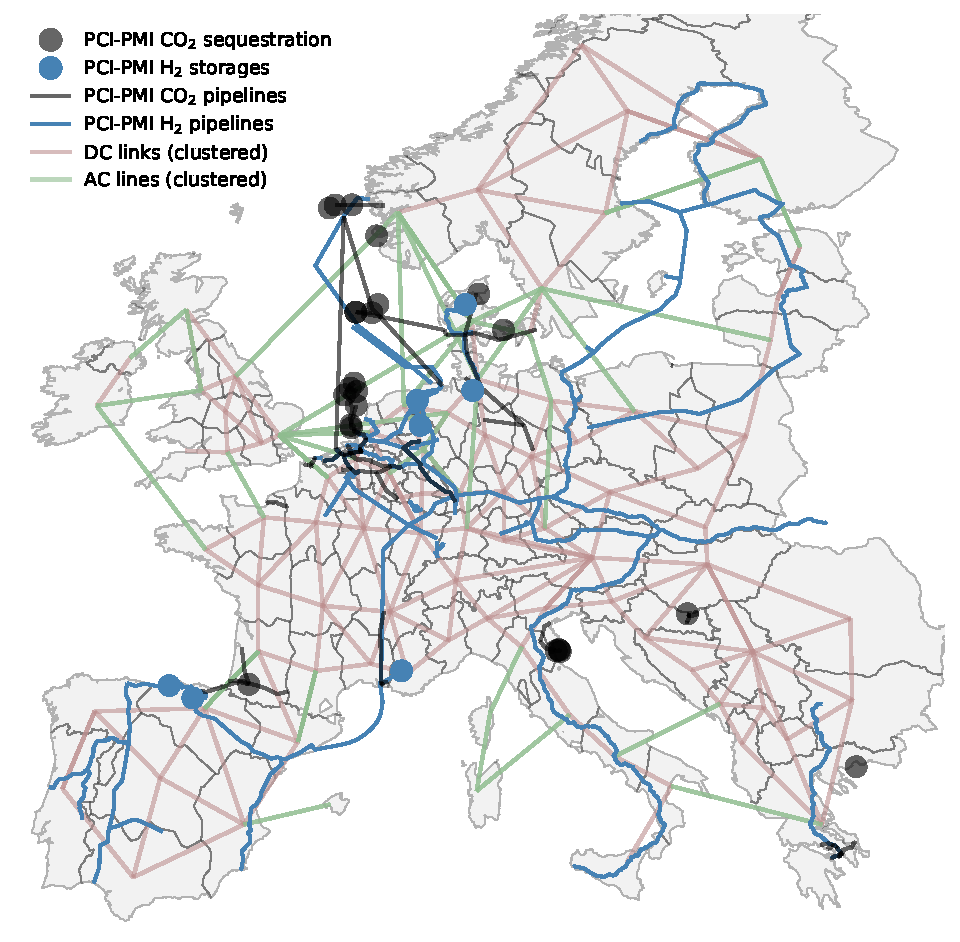
\includegraphics[width=1\textwidth]{pci_pmi_projects_map}
    \end{column}
  \end{columns}
  \source{Own illustration based on data extracted from \url{https://ec.europa.eu/energy/infrastructure/transparency_platform/map-viewer}}
\end{frame} 

\section{First results 2030}

\begin{frame}{First results: Base (All targets)}
  
  \centering

  \begin{columns}
    \begin{column}{0.5\textwidth}
      \footnotesize
      \begin{figure}
        \centering
        \includegraphics[width=0.72\textwidth]{baseline/maps/base_s_90_lv1.05__-balance_map_H2_2030.pdf}
      \end{figure}
    \end{column}
    \begin{column}{0.5\textwidth}
      \begin{figure}
        \centering
        \includegraphics[width=0.72\textwidth]{baseline/maps/base_s_90_lv1.05__-balance_map_co2_stored_2030.pdf}
      \end{figure}
    \end{column}
  \end{columns}
  \source{Own illustration.}

\end{frame}

\begin{frame}{First results: Scenario A. PCI-PMI delay (All targets)}
  
  \centering

  \begin{columns}
    \begin{column}{0.5\textwidth}
      \footnotesize
      \begin{figure}
        \centering
        \includegraphics[width=0.72\textwidth]{scenario_a_targets_no_pipelines/maps/base_s_90_lv1.05__-balance_map_H2_2030.pdf}
      \end{figure}
    \end{column}
    \begin{column}{0.5\textwidth}
      \begin{figure}
        \centering
        \includegraphics[width=0.72\textwidth]{scenario_a_targets_no_pipelines/maps/base_s_90_lv1.05__-balance_map_co2_stored_2030.pdf}
      \end{figure}
    \end{column}
  \end{columns}
  \source{Own illustration.}

\end{frame}

\begin{frame}{First results: Scenario B. PCI-PMI delay (Emission target only)}
  
  \centering

  \begin{columns}
    \begin{column}{0.5\textwidth}
      \footnotesize
      \begin{figure}
        \centering
        \includegraphics[width=0.72\textwidth]{scenario_b_no_targets_no_pipelines/maps/base_s_90_lv1.05__-balance_map_H2_2030.pdf}
      \end{figure}
    \end{column}
    \begin{column}{0.5\textwidth}
      \begin{figure}
        \centering
        \includegraphics[width=0.72\textwidth]{scenario_b_no_targets_no_pipelines/maps/base_s_90_lv1.05__-balance_map_co2_stored_2030.pdf}
      \end{figure}
    \end{column}
  \end{columns}
  \source{Own illustration.}

\end{frame}

\begin{frame}{First results: Total system costs}
  
  \centering
  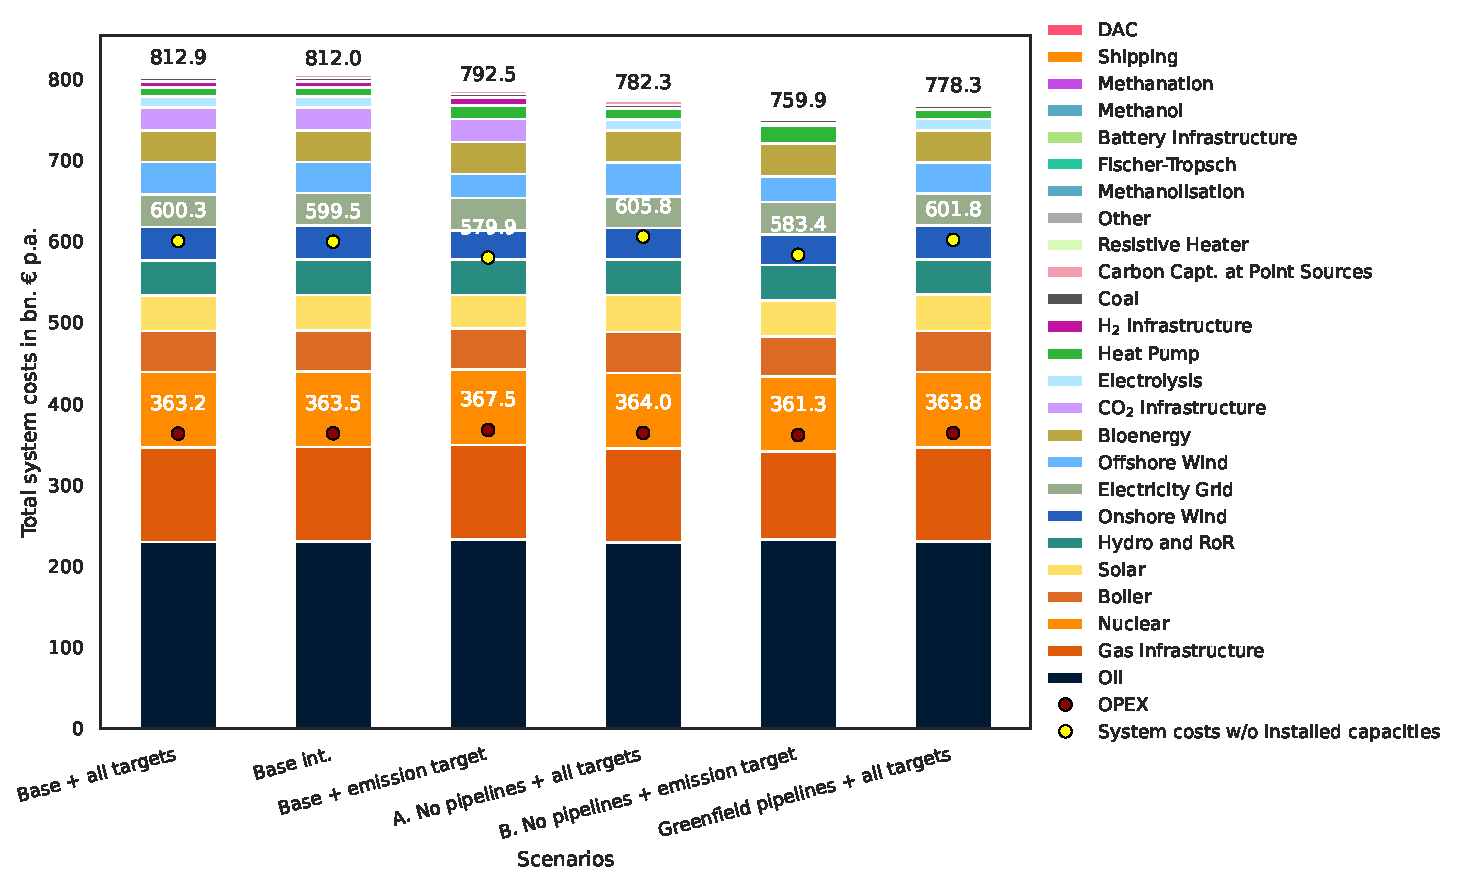
\includegraphics[height=0.75\paperheight]{system_costs}

  \source{Own illustration.}

\end{frame}


\begin{frame}{Case study: First takeaways for modelling year 2030}
  \footnotesize
  \begin{enumerate}
    \setlength\itemsep{0.3em}
      \item Reaching the EU's 2030 H$_2$ production and CO$_2$ sequestration targets translates into around \alert{20 bn. € p.a. in total system costs} for all included sectors, with or without PCI-PMI H$_2$ and CO$_2$ infrastructure projects.
      \item By omitting an H$_2$ target, almost no electrolysers are installed. \alert{Around 8 Mt of H$_2$} are still produced to cover industrial H$_2$ and methanol (primarily shipping) demand. Instead of through electrolysis, this demand is met by decentral steam methane reforming (SMR). 
      \item Setting a policy target may however be essential to \alert{kick-start the H$_2$ economy}. H$_2$ is then primarily created through electrolysis and used as a \alert{precursor} for methanolisation and to meet industrial demand. 
      \item Without specifying a CO$_2$ sequestration target, the system still captures and sequesters \alert{around 21 Mt of CO$_2$ p.a.} (primarily from process emissions).
      \item While all three \alert{EU policy targets for 2030 can still be achieved} without PCI-PMI infrastructure, they bring additional benefits:
      \begin{itemize}
        \footnotesize
        \item PCI-PMI H$_2$ pipelines help distribute more \alert{affordable green H$_2$} from northern and south-western Europe to high-demand regions central Europe
        \item PCI-PMI CO$_2$ pipelines connect \alert{industrial sites} and their process emissions to \alert{major offshore sequestration sites in the North Sea} (DK, NO, NL).
      \end{itemize}
  \end{enumerate}

\end{frame}


\section{Outlook and next steps}
\begin{frame}{Outlook}
  \footnotesize
  \begin{itemize}
    \item Including \alert{all relevant PCI-PMI projects}, i.e. hybrid offshore interconnectors (energy islands), electricity storages, CO$_2$ shipping routes
    \item Looking at the \alert{long-term value of PCI-PMI projects} in a sector-coupled European energy system through modelling pathways towards 2040 and 2050
    \item Incorporating technology-specific \alert{build-out rate limits} for earlier target years, e.g. for electrolysis
    \item Assessing the impact of \alert{sector-specific} PCI-PMI project delays
  \end{itemize}
\end{frame}
\begin{frame}
  \setbeamercolor{background canvas}{bg=red}
  \centering
  \fcolorbox{white}{tub-red}{\parbox[c][0.9\textheight][c]{\textwidth}{%
      \centering \color{white}\Large{\textbf{Thank you.}} \\ 
      \scriptsize
      \vspace{0.5cm}
      \href{https://github.com/pypsa/pypsa-eur}{\textcolor{white}{$\hookrightarrow$ github.com/pypsa/pypsa-eur}} \\
      \vspace{0.5cm}
      Department of\\\textbf{Digital Transformation in Energy Systems (ENSYS)} \\
      \vspace{0.5cm}
      \textbf{Bobby Xiong}\\
      \href{mailto:xiong@tu-berlin.de}{\textcolor{white}{$\hookrightarrow$ xiong@tu-berlin.de}} \\
      \href{https://github.com/bobbyxng}{\textcolor{white}{$\hookrightarrow$ github.com/bobbyxng}} \\
  }}
\end{frame}

% Appendix
\section{Appendix}

\begin{frame}
  \setbeamercolor{background canvas}{bg=red}
  \centering
  \fcolorbox{white}{tub-red}{\parbox[c][0.9\textheight][c]{\textwidth}{%
      \centering \color{white}\Large{\textbf{Appendix}}
  }}
\end{frame}

\begin{frame}{Case study: Sensitivity --- Base ext. (All targets)}
  
  \centering

  \begin{columns}
    \begin{column}{0.5\textwidth}
      \footnotesize
      \begin{figure}
        \centering
        \includegraphics[width=0.72\textwidth]{baseline_extended/maps/base_s_90_lv1.05__-balance_map_H2_2030.pdf}
      \end{figure}
    \end{column}
    \begin{column}{0.5\textwidth}
      \begin{figure}
        \centering
        \includegraphics[width=0.72\textwidth]{baseline_extended/maps/base_s_90_lv1.05__-balance_map_co2_stored_2030.pdf}
      \end{figure}
    \end{column}
  \end{columns}
  \source{Own illustration.}

\end{frame}
\begin{frame}{Case study: Sensitivity --- Greenfield Pipelines (All targets)}
  
  \centering

  \begin{columns}
    \begin{column}{0.5\textwidth}
      \footnotesize
      \begin{figure}
        \centering
        \includegraphics[width=0.72\textwidth]{targets_greenfield_pipelines/maps/base_s_90_lv1.05__-balance_map_H2_2030.pdf}
      \end{figure}
    \end{column}
    \begin{column}{0.5\textwidth}
      \begin{figure}
        \centering
        \includegraphics[width=0.72\textwidth]{targets_greenfield_pipelines/maps/base_s_90_lv1.05__-balance_map_co2_stored_2030.pdf}
      \end{figure}
    \end{column}
  \end{columns}
  \source{Own illustration.}

\end{frame}

\begin{frame}{First results: Total system costs}
  
  \centering
  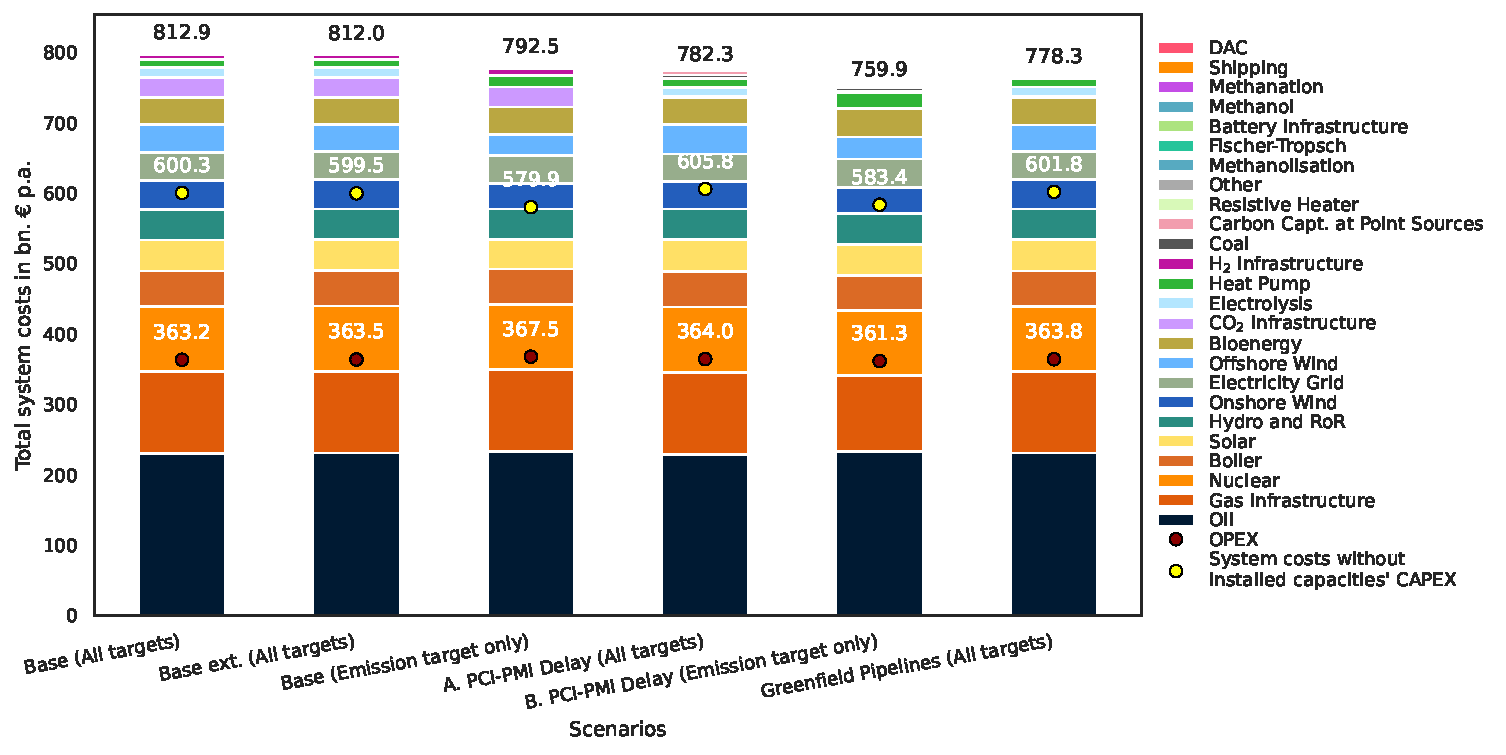
\includegraphics[height=0.75\paperheight]{system_costs_all}

  \source{Own illustration.}

\end{frame}

\begin{frame}{First results: Hydrogen balance}
  
  \centering
  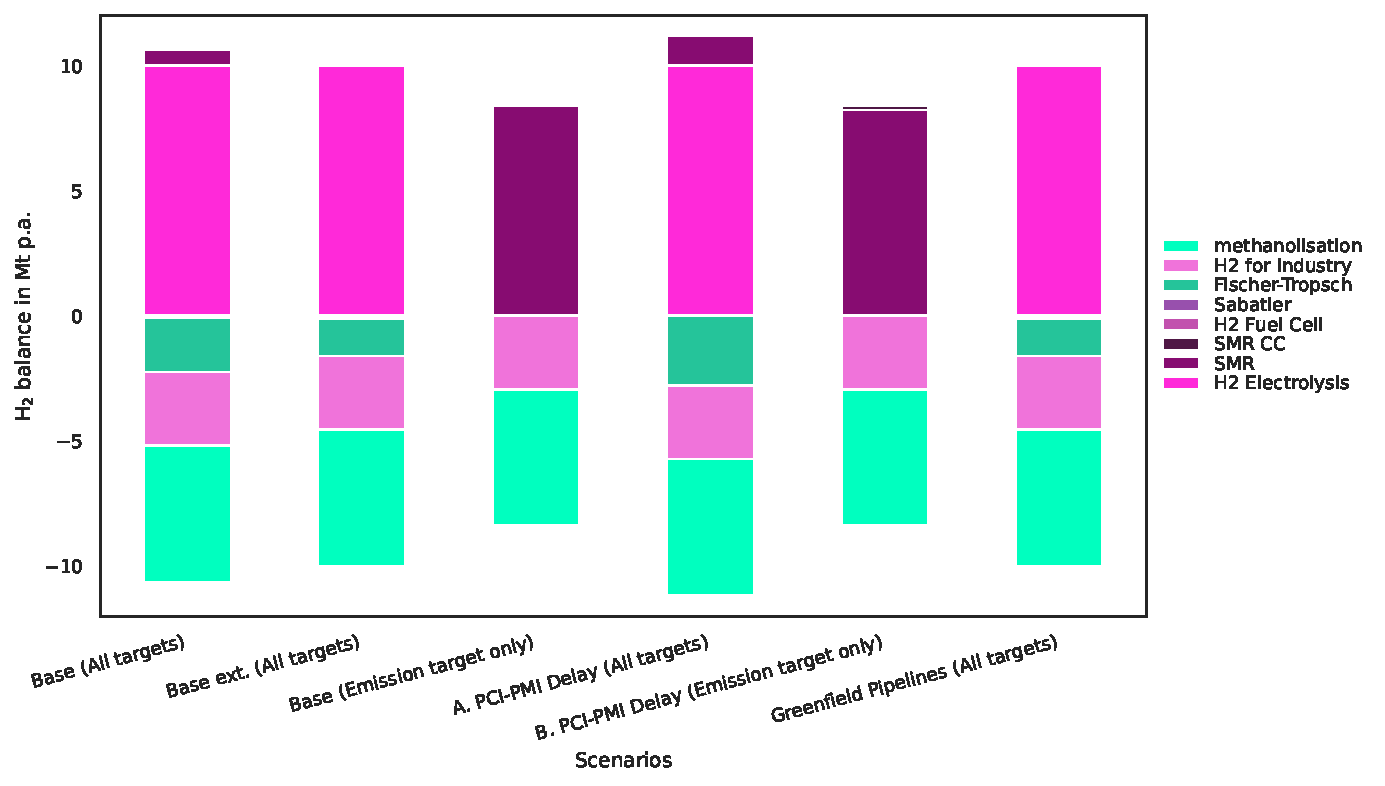
\includegraphics[height=0.75\paperheight]{h2_balance_all}

  \source{Own illustration.}
\end{frame}

\begin{frame}{First results: Carbon balance}
  \centering
  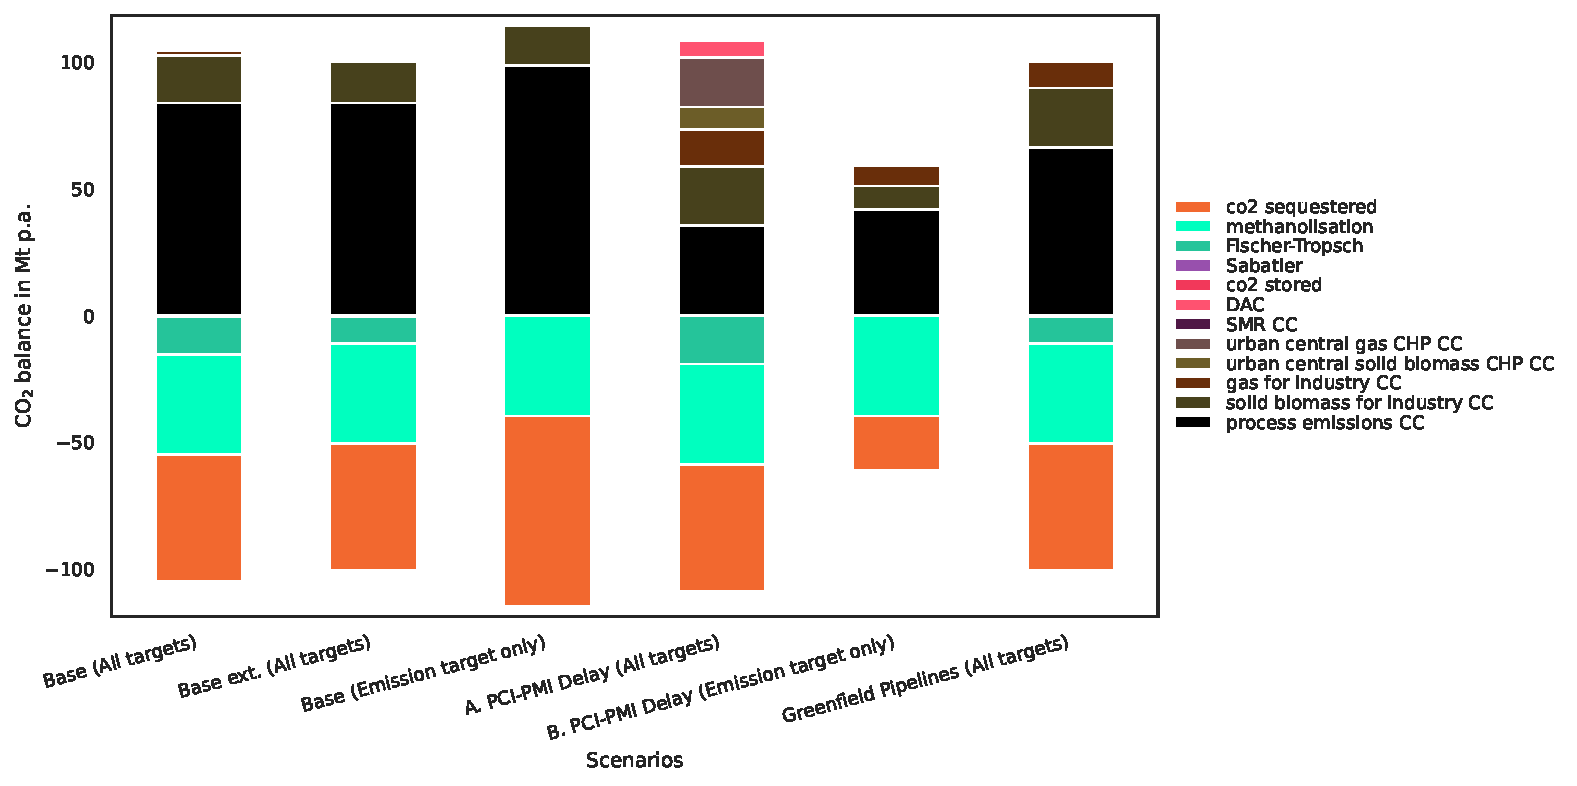
\includegraphics[height=0.75\paperheight]{co2_stored_balance_all}

  \source{Own illustration.}

\end{frame}

\begin{frame}{First results: Methanol balance}
  
  \centering
  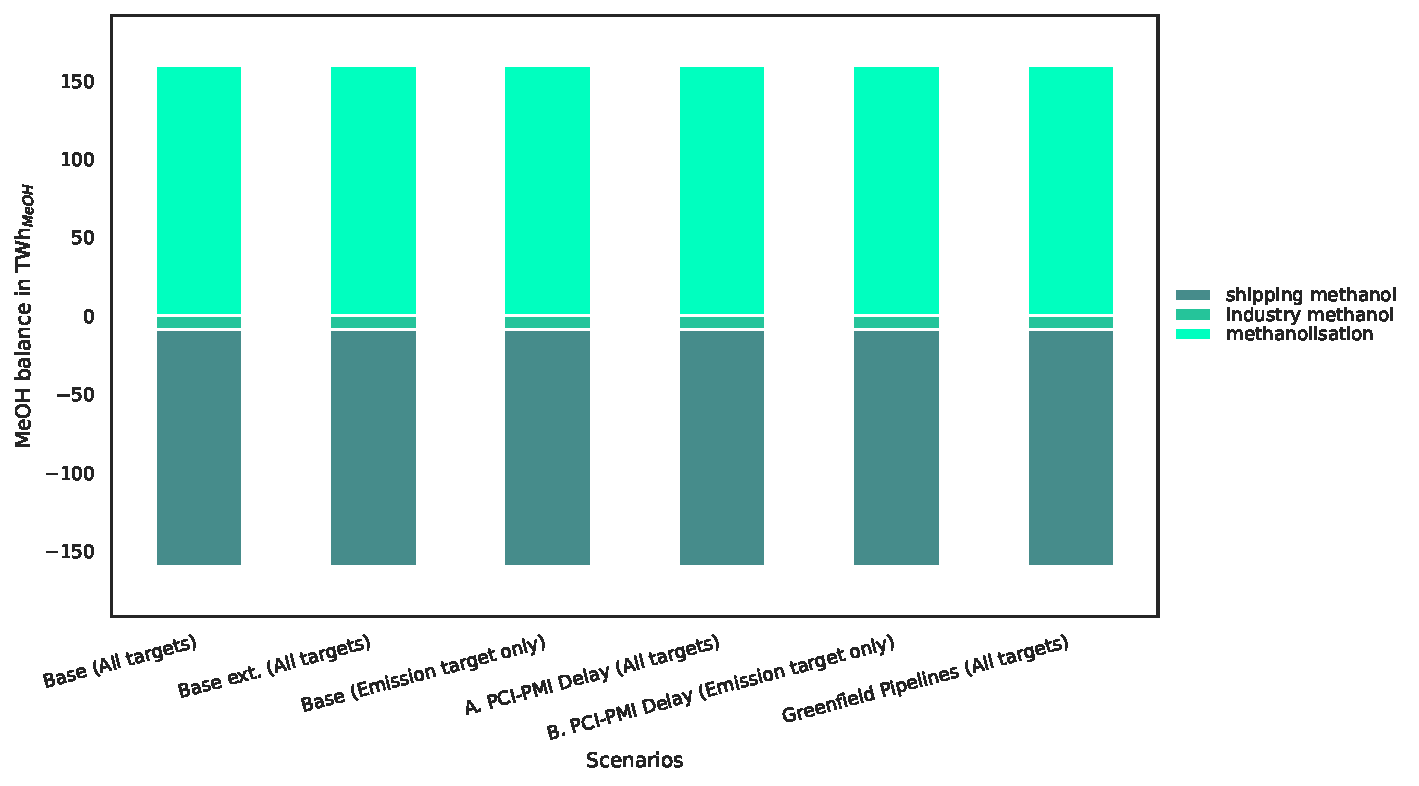
\includegraphics[height=0.75\paperheight]{methanol_balance_all}

  \source{Own illustration.}

\end{frame}



\begin{frame}{\textbf{Why H$_2$?} Most H$_2$ is used for derivative fuels and chemicals!}
  
  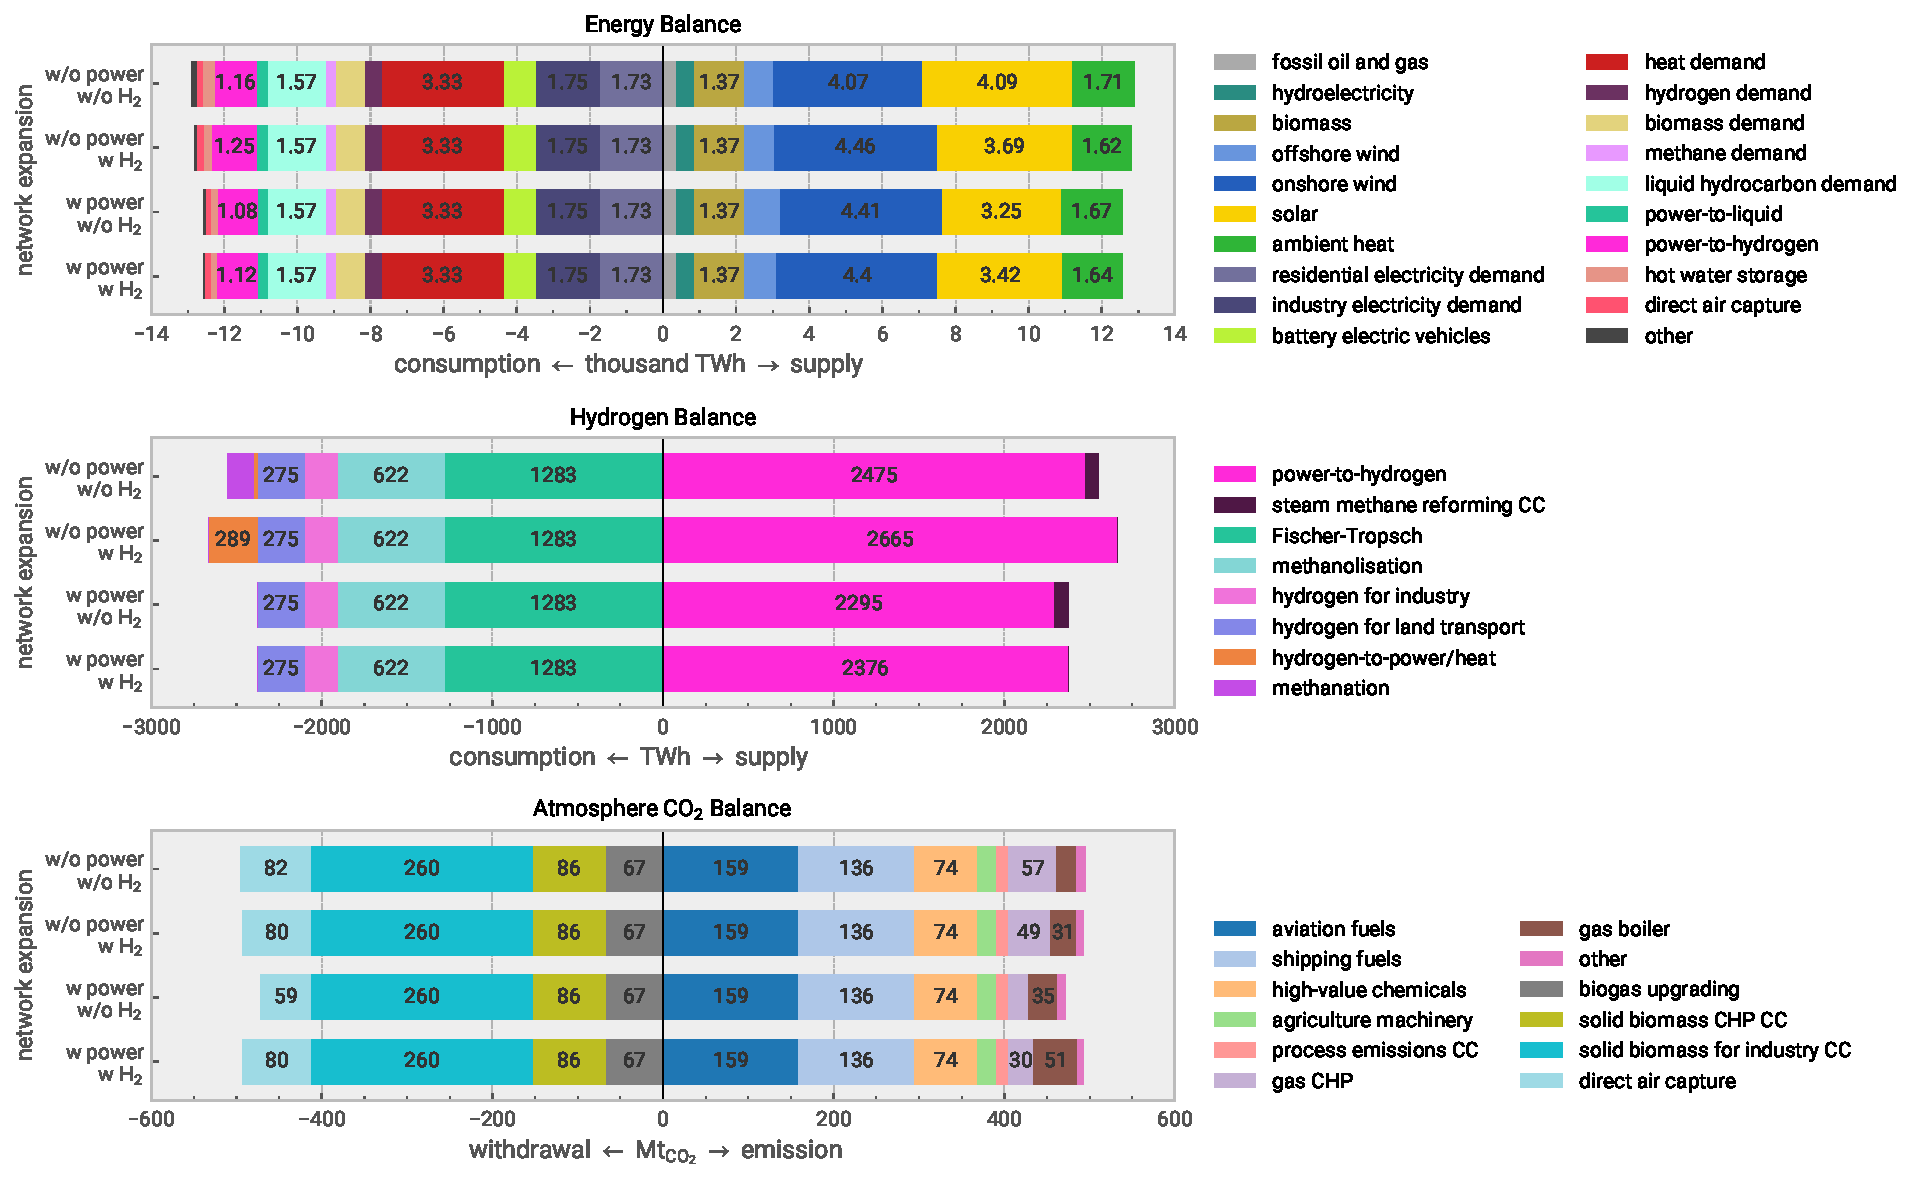
\includegraphics[width=1.2\textwidth, trim=0cm 6.6cm 0cm 6.6cm, clip]{other/hydrogen_balance.pdf}

  \footnotesize

  Mostly \alert{green electrolytic hydrogen supply}. \alert{Few direct uses of hydrogen} in the energy system, but it is
  used to synthesise other fuels and chemicals:

  \begin{multicols}{2}
  \begin{itemize}
    \item ammonia for fertilizers
    \item direct reduced iron for steelmaking
    \item shipping and aviation fuels
    \item precursor to high-value chemicals
    \item backup heat and power supply
    \item some heavy duty land transport
  \end{itemize}
  \end{multicols}

  \source{Neumann, Zeyen, Victoria, Brown, 2023\\\url{https://doi.org/10.1016/j.joule.2023.06.016}}
\end{frame}

\begin{frame}{Transporting \textbf{CO$_2$ to H$_2$} or transporting \textbf{H$_2$ to CO$_2$}?}
  
  \centering
  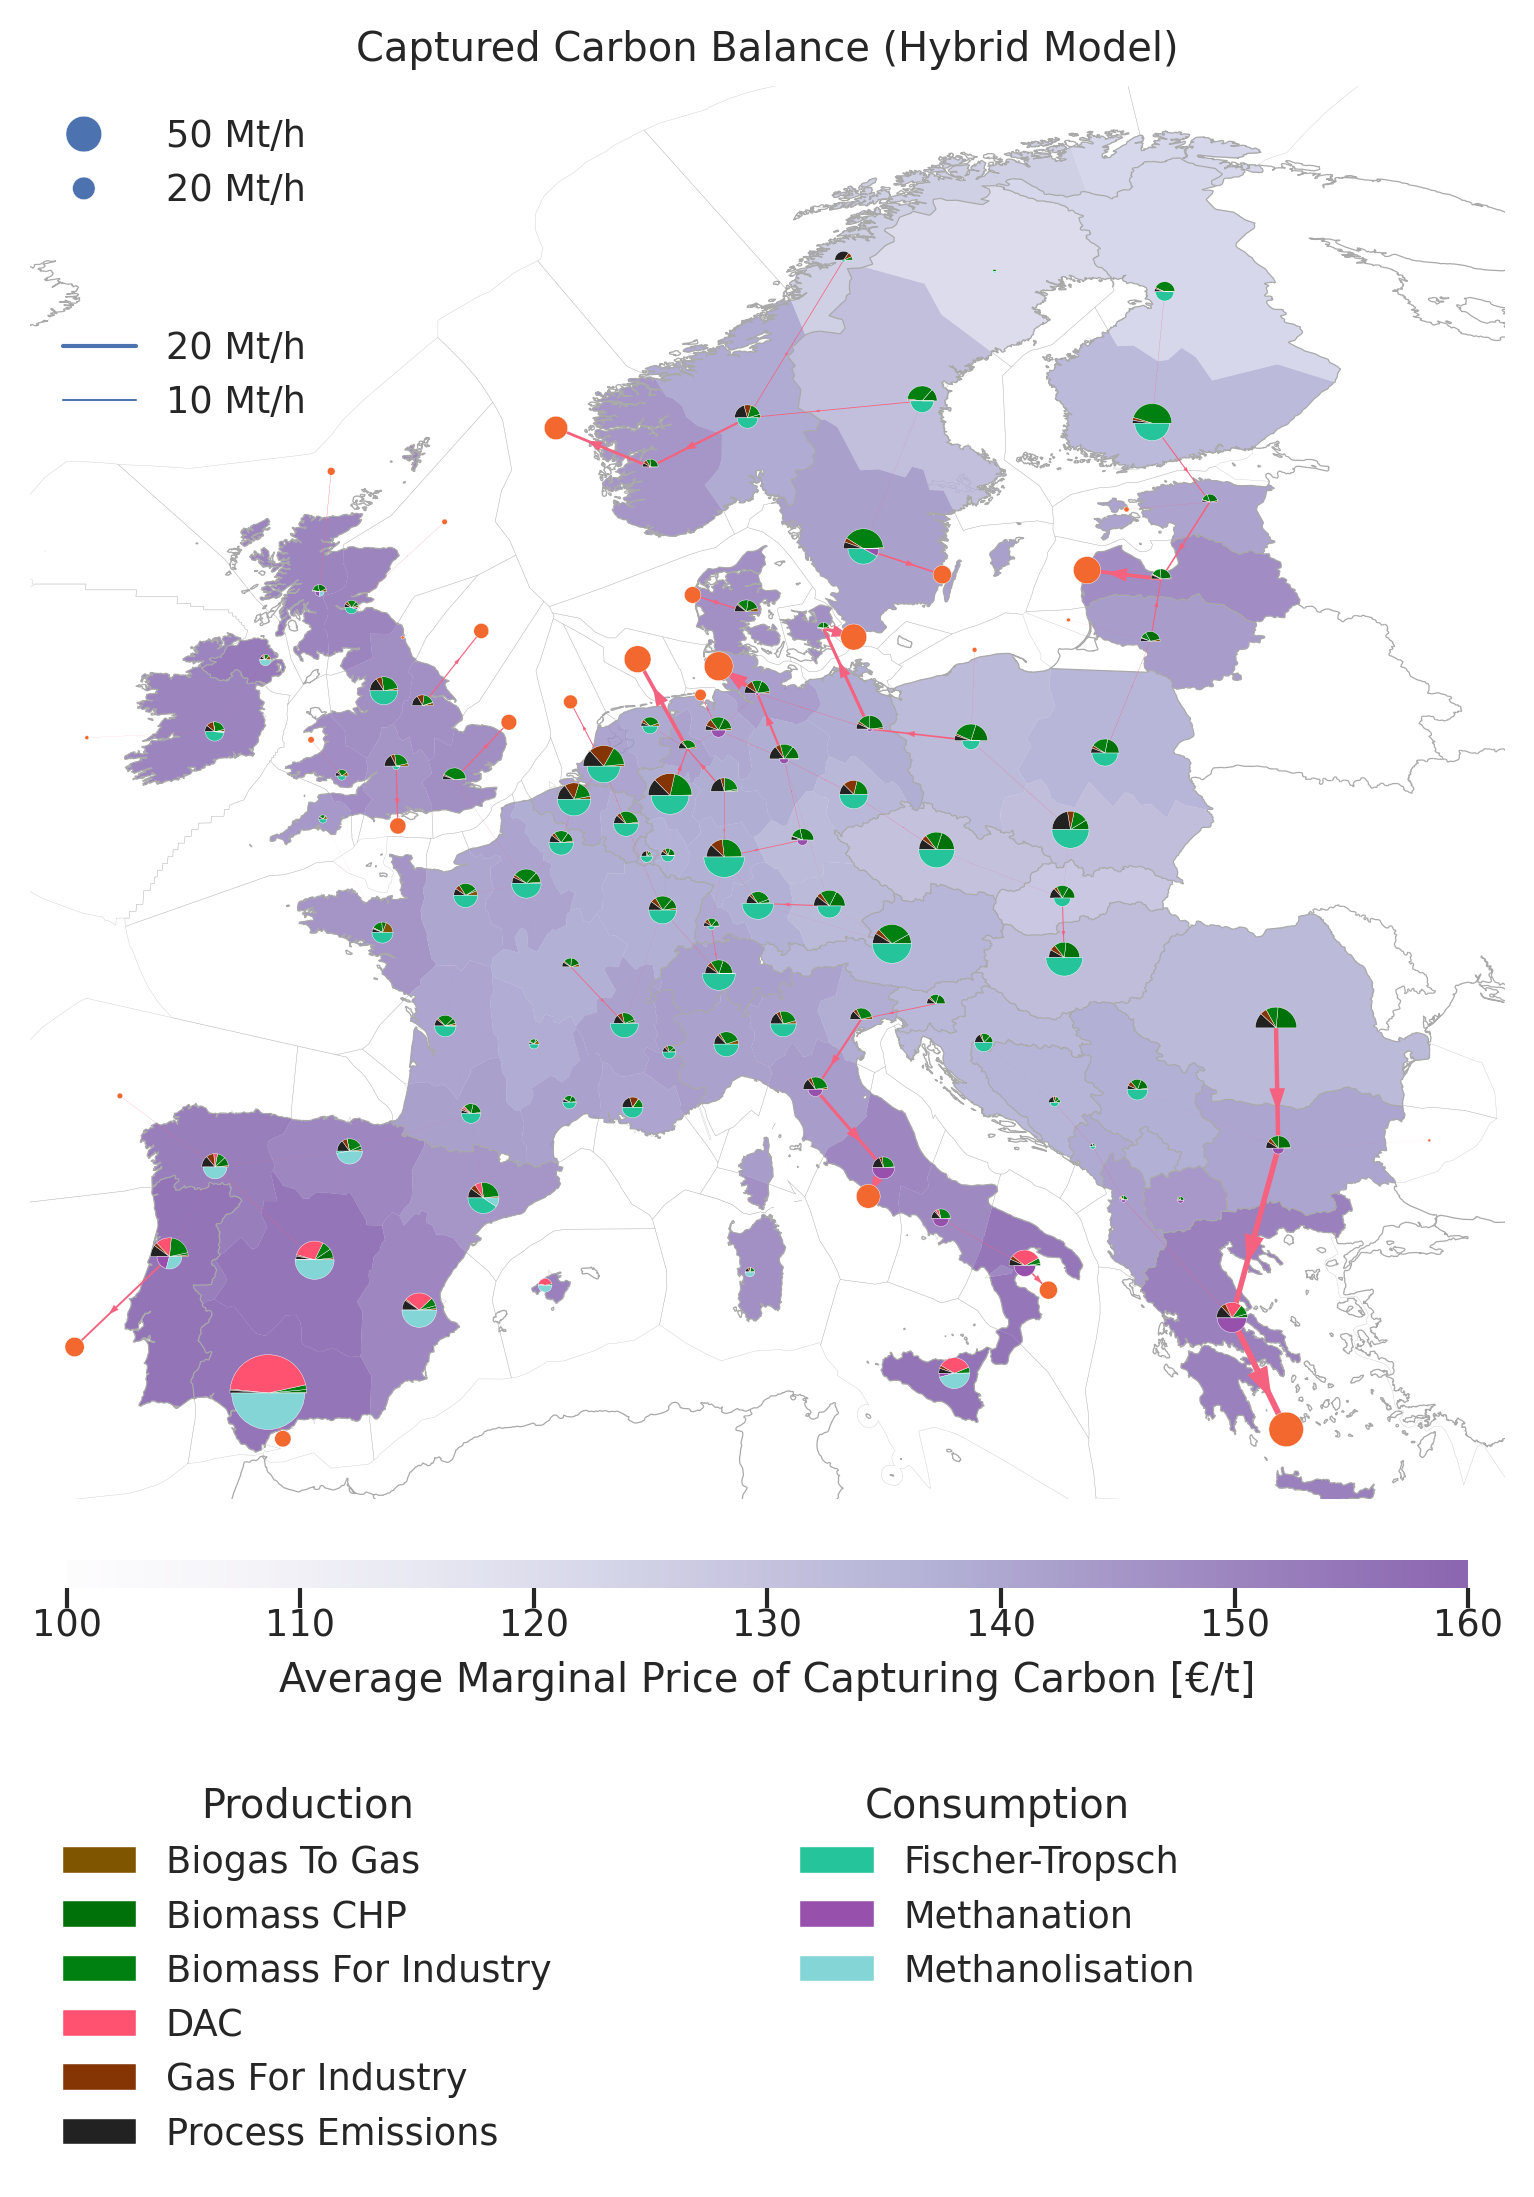
\includegraphics[width=0.35\textwidth]{other/carbon_networks_balance_map_carbon}
  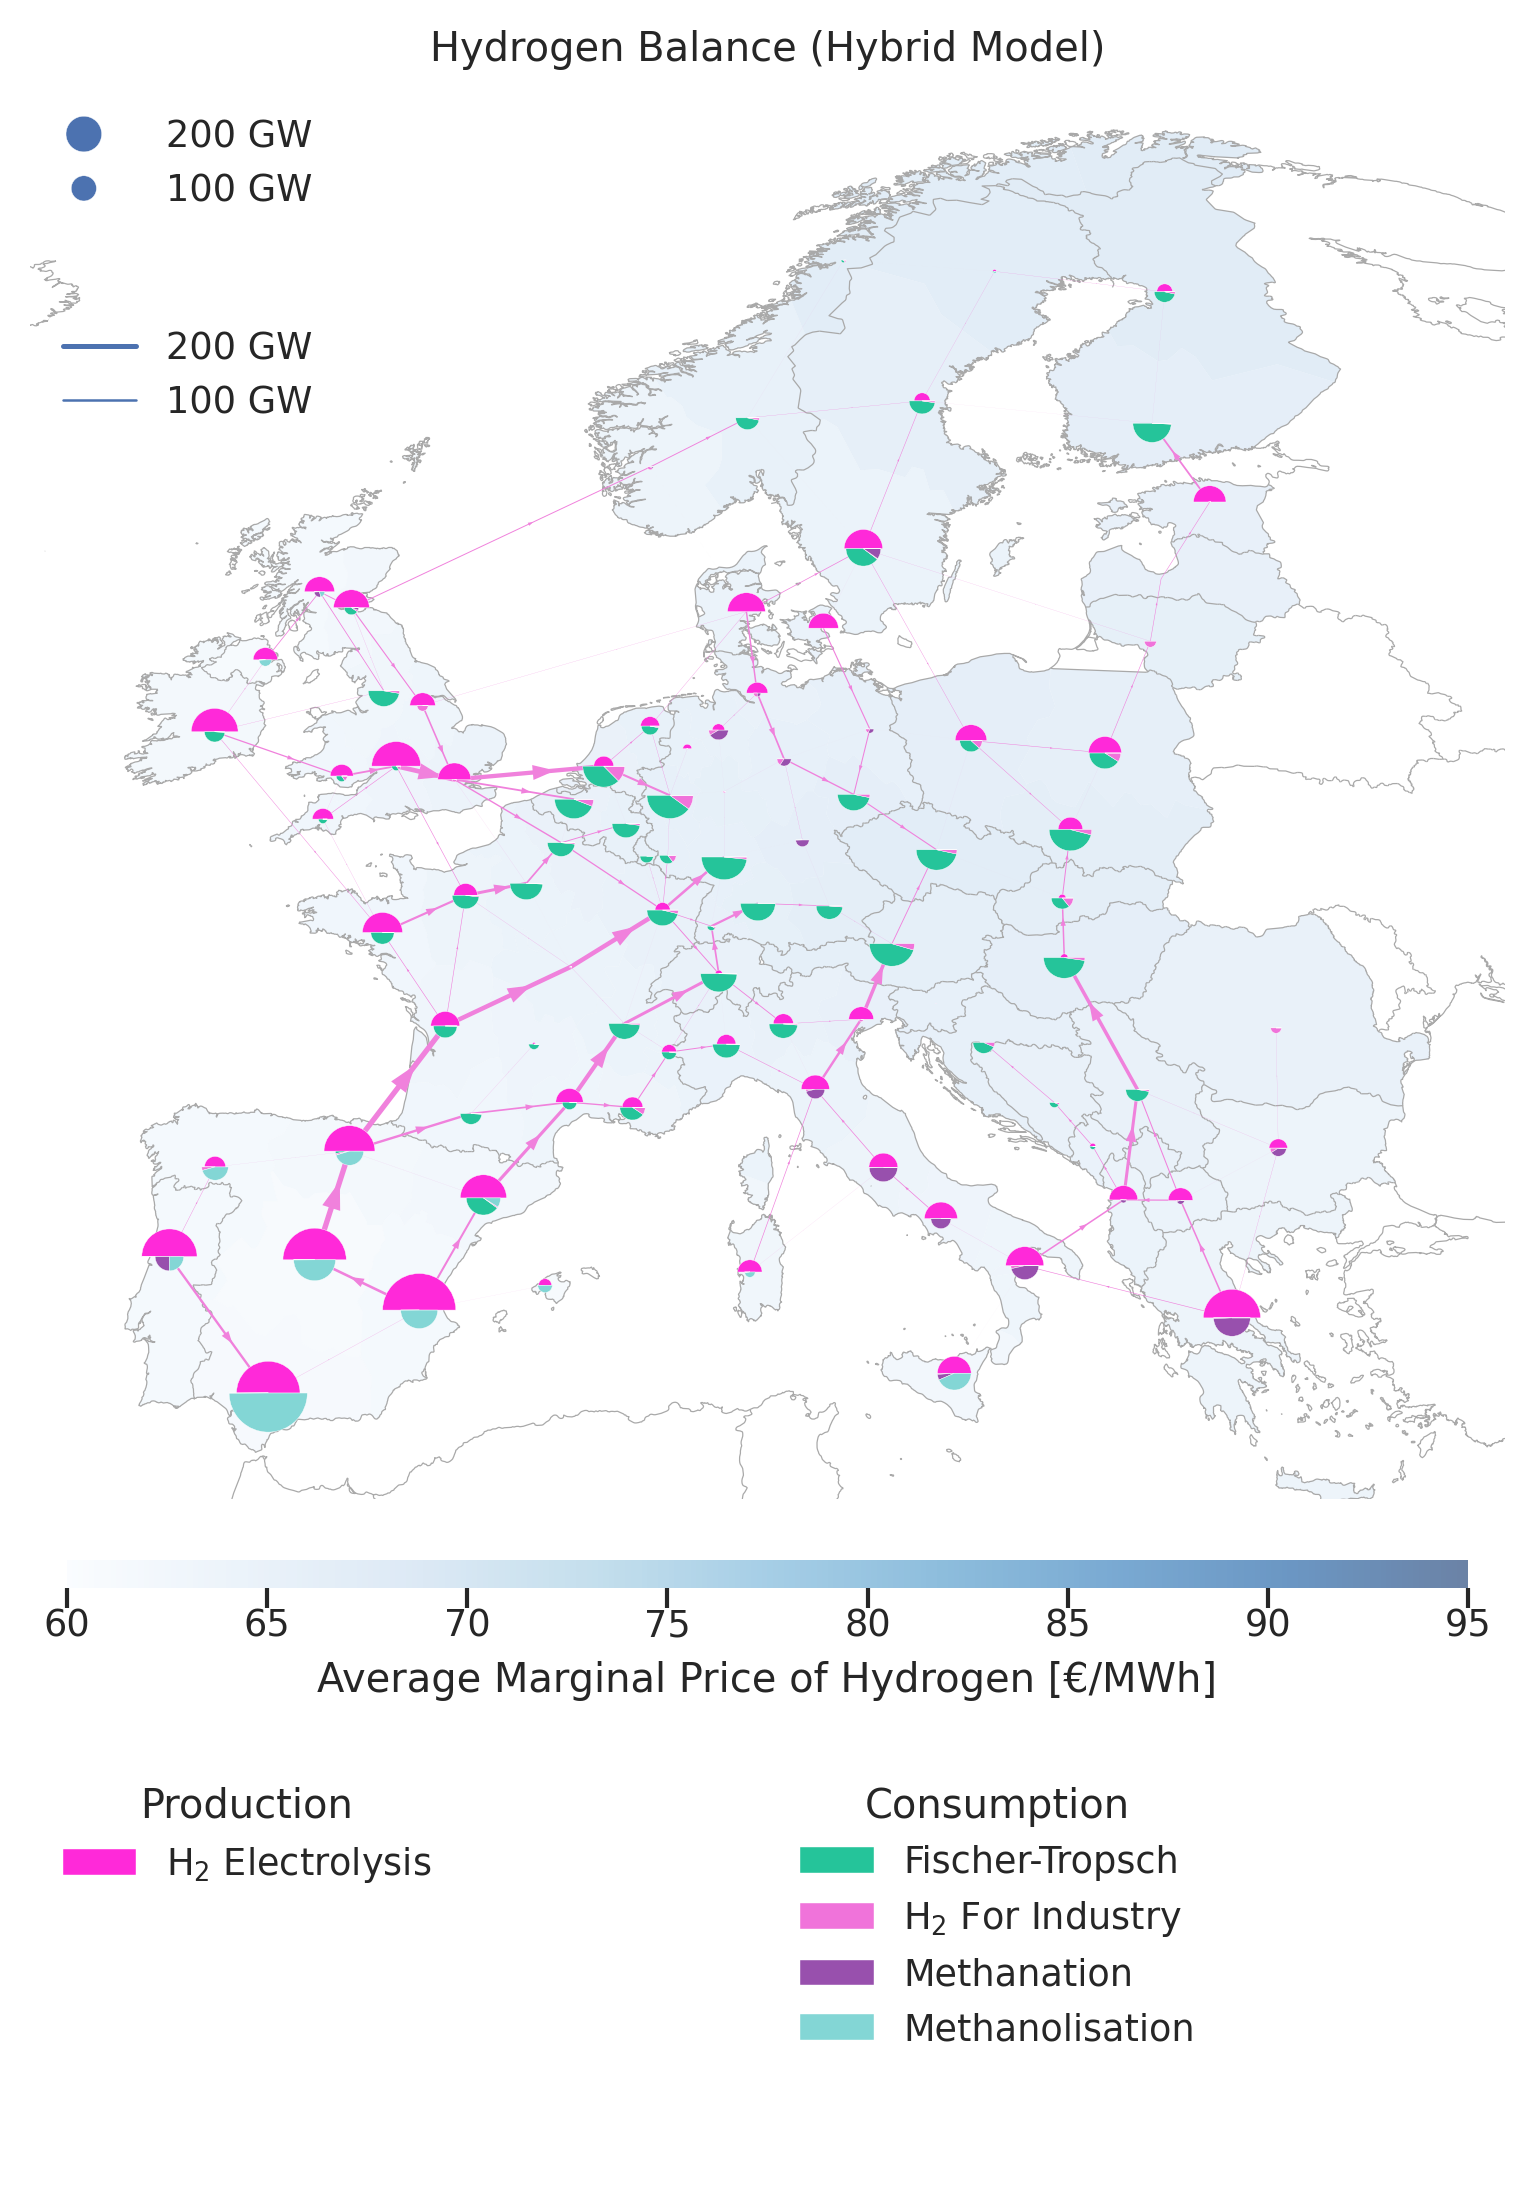
\includegraphics[width=0.35\textwidth]{other/carbon_networks_balance_map_hydrogen}

  \source{Hofmann, Tries, Neumann, Zeyen, Brown, 2024\\\url{https://arxiv.org/abs/2402.19042}}

\end{frame}


\begin{frame}{\textbf{Carbon management}: Capture, use, transport and sequestration}
  
  \begin{center}
    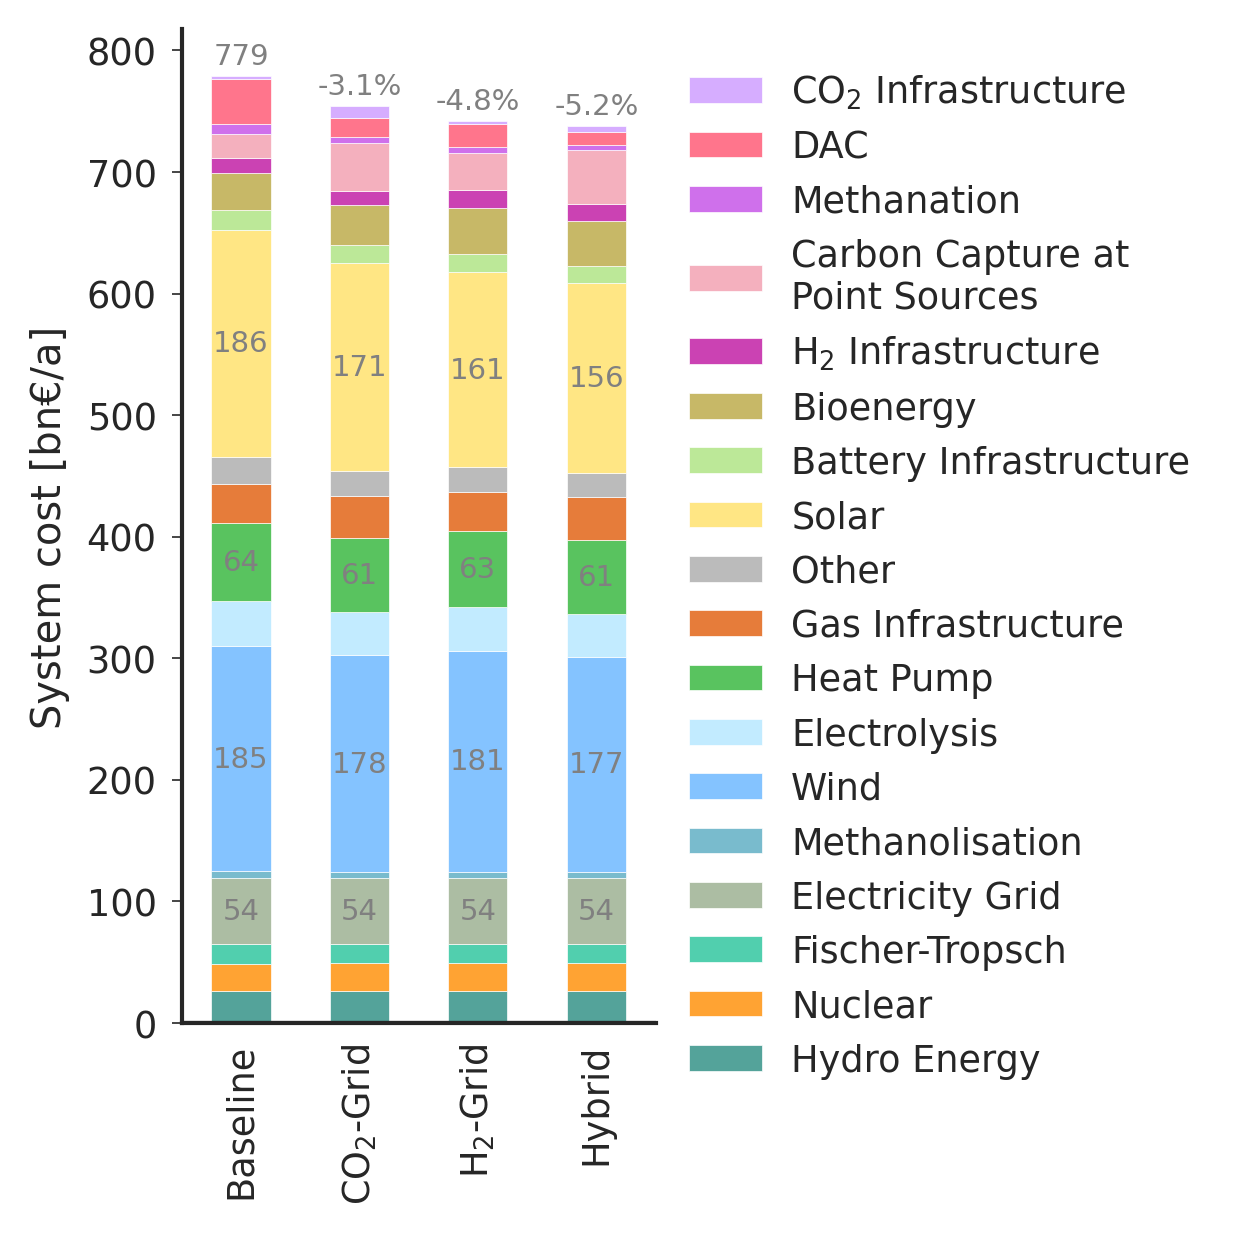
\includegraphics[height=0.73\textheight]{other/carbon_networks_cost_bar}
    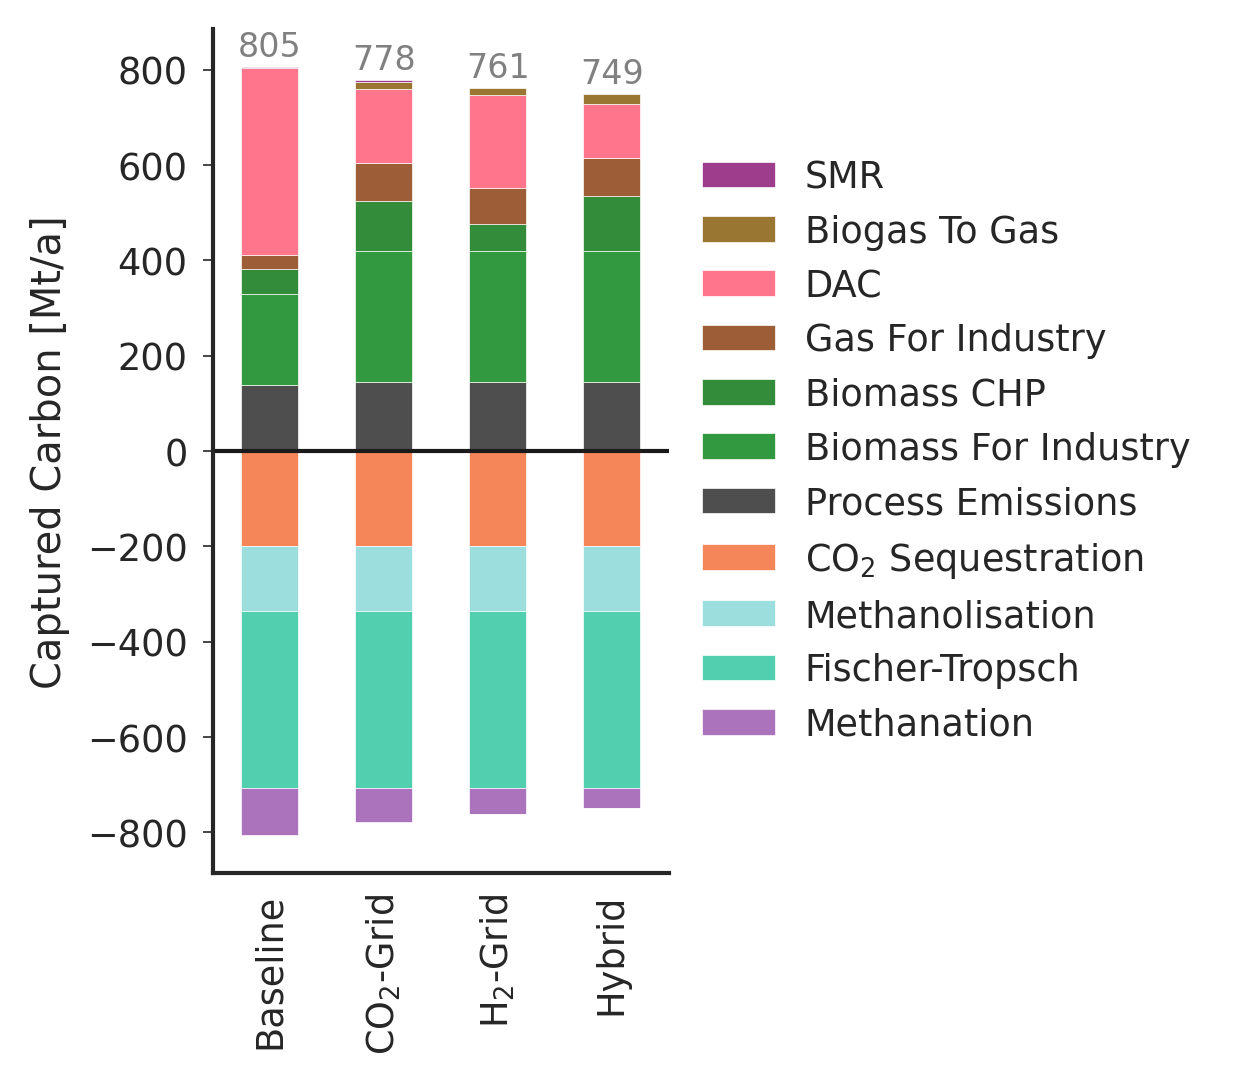
\includegraphics[height=0.71\textheight]{other/carbon_networks_balance_bar_carbon}

    \vspace{-0.25cm}
    \footnotesize
    \begin{itemize}
      \item \alert{CCS} for process emissions (for instance, in cement industry)
      \item \alert{CCU} for e-synfuels and e-chemicals (in particular, shipping, aviation, plastics)
      \item \alert{CDR} for unabatable and negative emissions (to offset imperfect capture rates)
    \end{itemize}

  \end{center}

  \source{Hofmann, Tries, Neumann, Zeyen, Brown, 2024\\\url{https://arxiv.org/abs/2402.19042}}

\end{frame}

\begin{frame}{Maximum sequestration potential}
  
  \begin{center}
    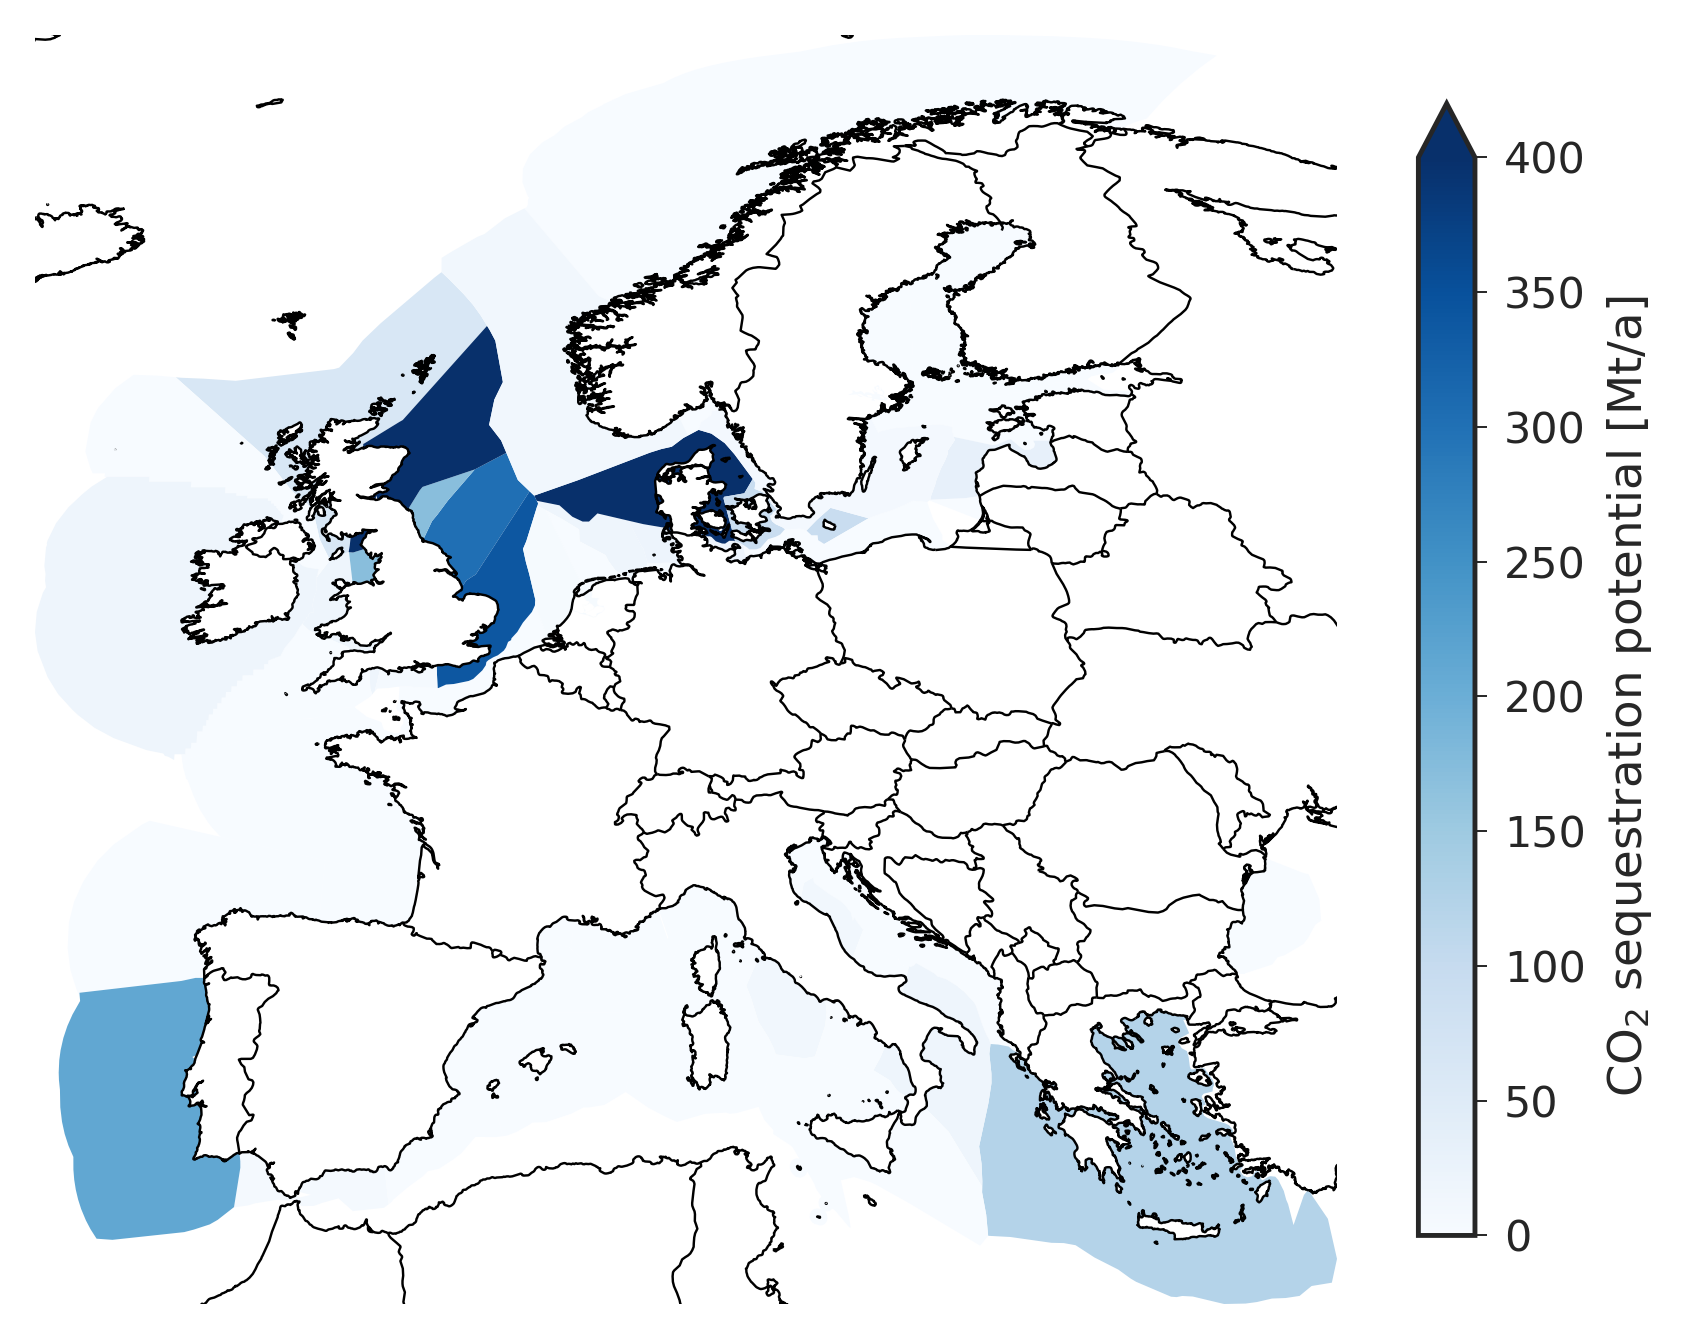
\includegraphics[height=0.9\textheight]{other/sequestration_map}

  \end{center}

  \source{Hofmann, Tries, Neumann, Zeyen, Brown, 2024\\\url{https://arxiv.org/abs/2402.19042}}

\end{frame}

\begin{frame}{Electricity high-voltage grid based on OpenStreetMap (OSM)}

  \begin{columns}
    \begin{column}{0.64\textwidth}
      \footnotesize
      \begin{itemize}
        \setlength\itemsep{.8em}
        \item Dataset contains a topologically connected representation of the European high-voltage grid (220 kV to 750 kV) constructed using OpenStreetMap data
        \item Heuristic cleaning process was used to for lines and links where electrical parameters are incomplete, missing, or ambiguous
        \item Close substations within a radius of 500 m are aggregated to single buses
        \item Unique transformers are added for each voltage pair in a substation
        \item AC lines mapped using pandapower's standard line type library. In default version, nominal capacity is set to 70 \% of the technical capacity to account for n-1 security approximation
        \item Includes all 38 European HVDC connections with their nominal rating that are commissioned as of 2024
      \end{itemize}
    \end{column}
    \begin{column}{0.36\textwidth}
      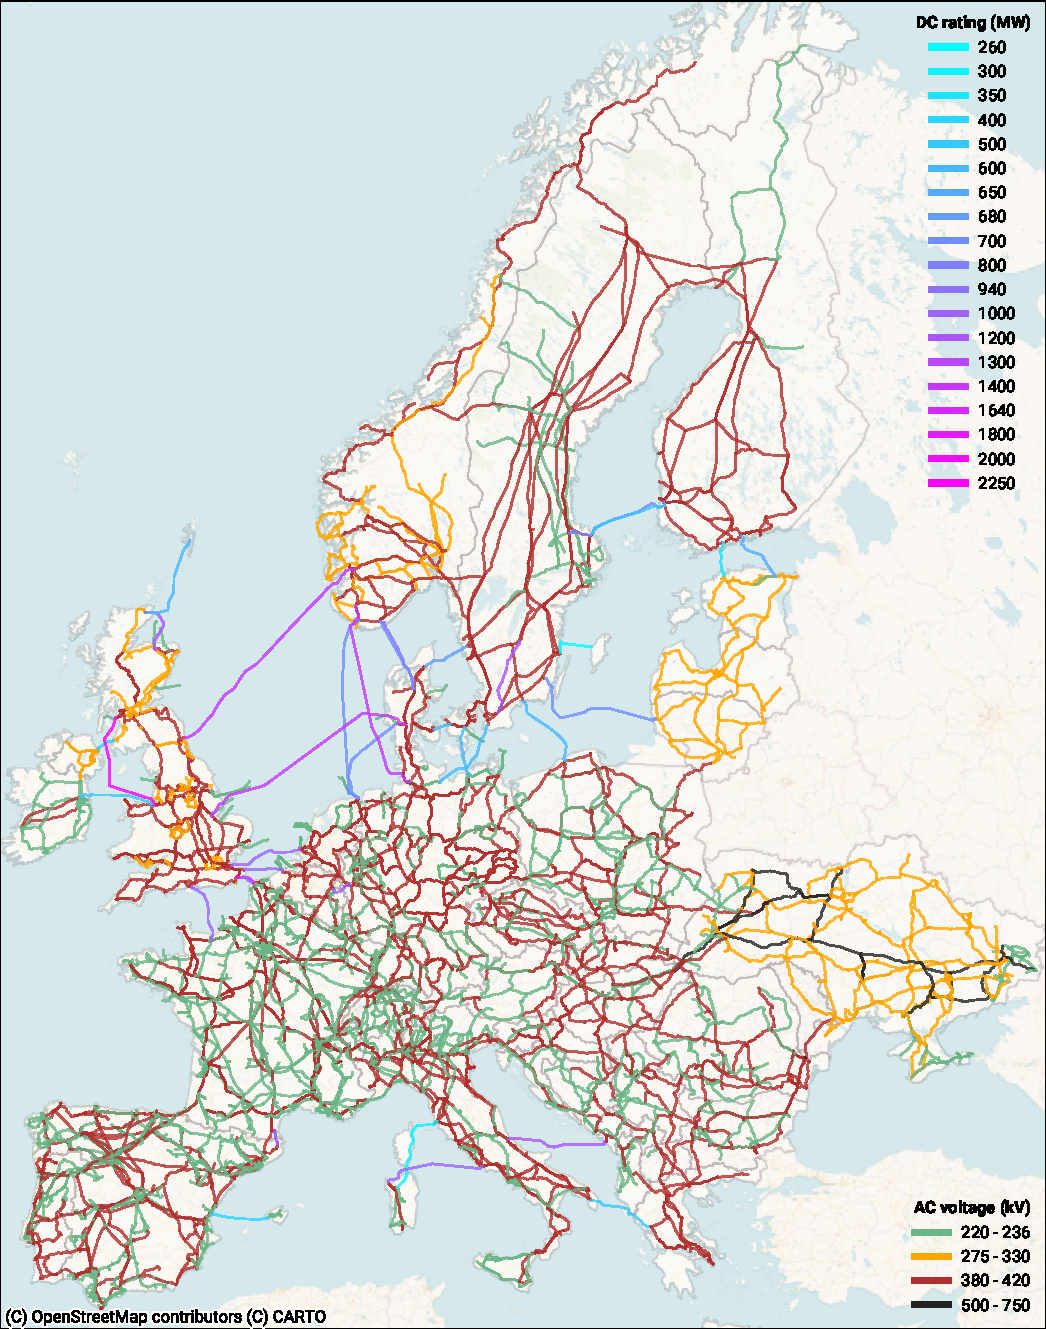
\includegraphics[width=1\textwidth]{osm_map}
    \end{column}
  \end{columns}
  \source{Own illustration based on data extracted using Overpass Turbo API\\\url{https://openstreetmap.org}}
  
  
\end{frame}

\end{document}